\PassOptionsToPackage{quiet}{fontspec}
\documentclass[12pt,a4paper,UTF8]{article}
\usepackage{thesis} % 格式控制
\usepackage{xeCJK}
\setCJKmainfont{SimSun}[AutoFakeBold=true] % 设置中易宋体为默认CJK字体
\usepackage{indentfirst}
\usepackage{float}
\setlength{\parindent}{2em} % 控制首行缩进  
\addtolength{\parskip}{3pt} % 控制段落距离  
\onehalfspacing % 1.5倍行距  
\graphicspath{{./figures/}} % 指定图片所在文件夹  


\classname{电磁场与电磁波实验}  % 设置课程名称
\makepagestyle{}{\printclassname ~实验报告}

\begin{document}
\maketitlepage{天线CST仿真实验}{东4-421}{郑智瑄}{3230103913}{\today}{王子立} %封面页 

\maketoc    %目录页

\section{实验目的}
\begin{enumerate}
  \item 矩形波导馈电角锥喇叭天线CST仿真
  \item 熟悉 CST 软件的基本使用方法，并能够运用其对特定的微波器件或电路进行建模、仿真分析。  
\end{enumerate}
\section{实验原理}
\subsection{喇叭天线概述}
喇叭天线是一种应用广泛的微波天线，其优点是结构简单、频带宽、功率容量
大、调整与使用方便。合理的选择喇叭尺寸，可以取得良好的辐射特性：相当尖
锐的主瓣，较小副瓣和较高的增益。因此喇叭天线在军事和民用上应用都非常广
泛，是一种常见的测试用天线。喇叭天线的基本形式是把矩形波导和圆波导的开
口面逐渐扩展而形成的，由于是波导开口面的逐渐扩大，改善了波导与自由空间
的匹配，使得波导中的反射系数小，即波导中传输的绝大部分能量由喇叭辐射出
去，反射的能量很小。实际的矩形波导馈电的角锥喇叭天线如图4-1所示。
\begin{figure}[H]
  \centering
  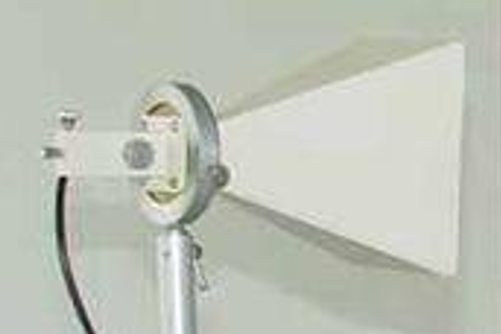
\includegraphics[width=0.65\linewidth]{figures/p1.png} % 数字表示放缩比例
  \caption{实际天线图} % 图片标题
\end{figure}
\subsection{喇叭天线分类}
\begin{figure}[H]
  \centering
  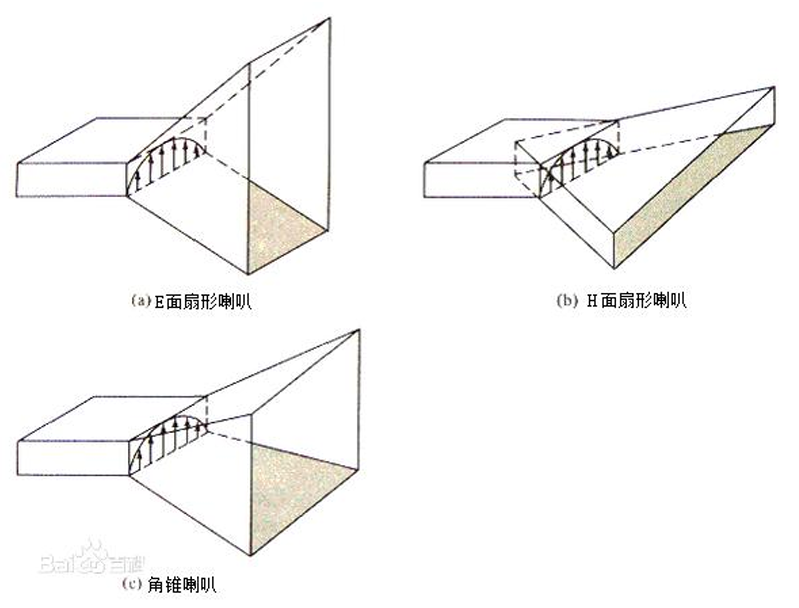
\includegraphics[width=0.65\linewidth]{figures/p2.png} % 数字表示放缩比例
  \caption{三种矩形波导馈电角锥喇叭天线的结构示意图} % 图片标题
\end{figure}
\subsection{尺寸确定}
角锥喇叭天线是对馈电的矩形波导在宽边和窄边均按一定的角度张开的，结构示意图如图3所示。矩形波导的尺寸为 $a \times b$，喇叭口径尺寸为 $D_H \times D_E$，喇叭高度为 $L$，其 $H$ 面（$xz$ 面）内虚顶点到口径中点的距离为 $R_1$，$E$ 面（$yz$ 面）内虚顶点到口径中心的距离为 $R_2$。

\begin{figure}[H]
  \centering
  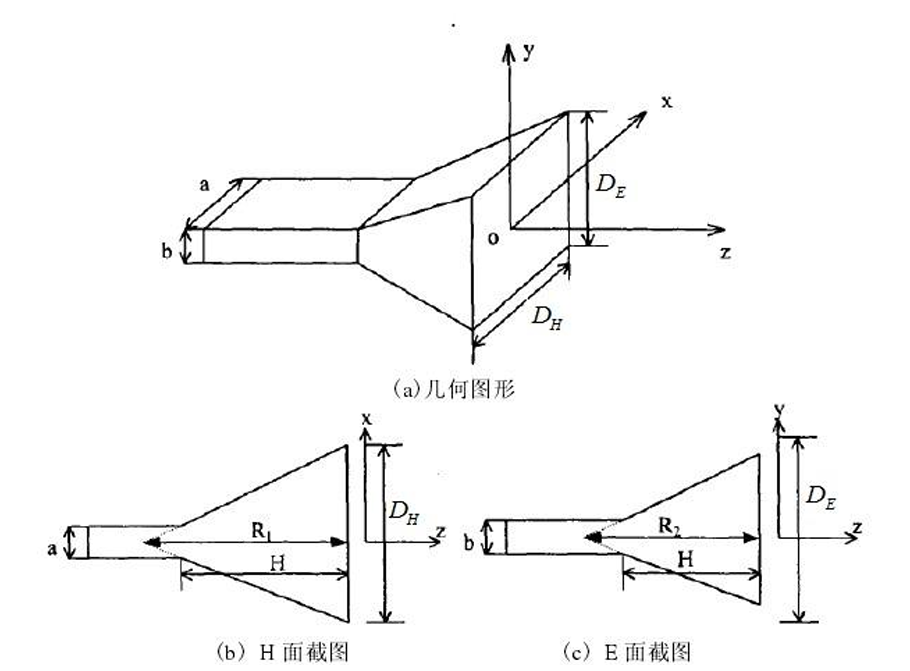
\includegraphics[width=0.65\linewidth]{figures/p3.png} % 数字表示放缩比例
  \caption{角锥喇叭天线的结构示意图} % 图片标题
\end{figure}

\subsection{理论分析}

对于矩形波导的尺寸为 $a\times b$，喇叭口径尺寸为 $A = D_H\times D_E$，喇叭高度为 $L$ 的角锥喇叭天线。可以用以下公式来估算该天线的增益：
$$
G=10.8+10\lg(D_{H}\times D_{E}/\lambda^{2})-\Delta G_{H}-\Delta G_{E}(dB)
$$

$\Delta G_{\mathrm{H}},~\Delta G_{\mathrm{E}}$,可以由查表得到，其中参数$\alpha , \beta $,可由公式求得。

$$
R_{_1}=\frac{L\times D_{_H}}{D_{_H}-a}
$$

$$
R_{_2}=\frac{L\times D_{_E}}{D_{_E}-b}
$$

$$
L_{H}=\sqrt{R_{1}^{2}+\frac{D_{H}^{2}}{4}}
$$

$$
L_{E}=\sqrt{R_{2}^{2}+\frac{D_{E}^{2}}{4}}
$$

$$
S_{_H}=A^{2}/(8\lambda L_{_H})
$$

$$
S_{E}=A^{2}/(8\lambda L_{E})
$$

$$
\alpha=8S_{H}
$$

$$
\beta=8S_{E}
$$

\begin{figure}[H]
  \centering
  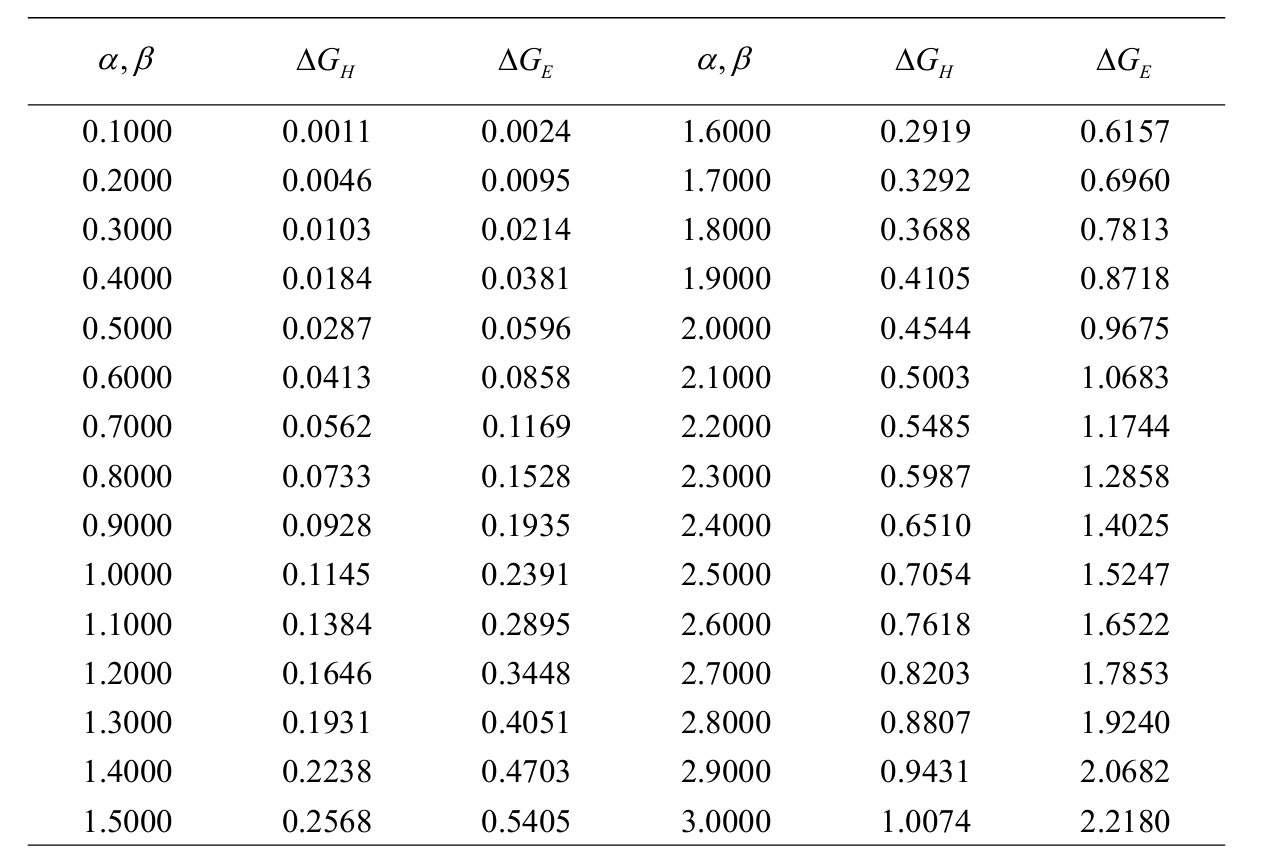
\includegraphics[width=0.65\linewidth]{figures/p4.jpg} % 数字表示放缩比例
  \caption{$\Delta G_{\mathrm{H}},~\Delta G_{\mathrm{E}}$数值表} % 图片标题
\end{figure}

\section{建模与仿真步骤}
\subsection{仿真步骤}
\begin{enumerate}
    \item \textbf{CST 初始设置}\\
    打开 CST 软件，选择 \texttt{New Project->MICROWAVES\&RF->Antennas->Waveguide (Horn,Cone,etc.)->Time Domain->Dimensions:mm;Frequency:GHz;}
    
    \item \textbf{建立模型}
    \begin{enumerate}
        \item 参数设置:
        \begin{table}[ht]
        \centering
        \caption{建模参数表}
        \label{tab:param}
        \begin{tabular}{cc}
        \toprule
        Parameter & Value(mm) \\
        \midrule
        $D_E$ & 38 \\
        $D_H$ & 80 \\
        L & 80 \\
        Lambda & 29.1 \\
        a & 22.86 \\
        b & 10.16 \\
        t & 1 \\
        \bottomrule
        \end{tabular}
        \end{table}
        
        \item 创建矩形波导：
        \begin{itemize}
          \item 点击 \texttt{Modeling->Shape->Brick}，按 Esc 键弹出参数窗口。
		  Layer 选择 \texttt{PEC}。
          \item 完成后的矩形波导模型如Figure 5所示。
          \begin{figure}[H]
			\centering
			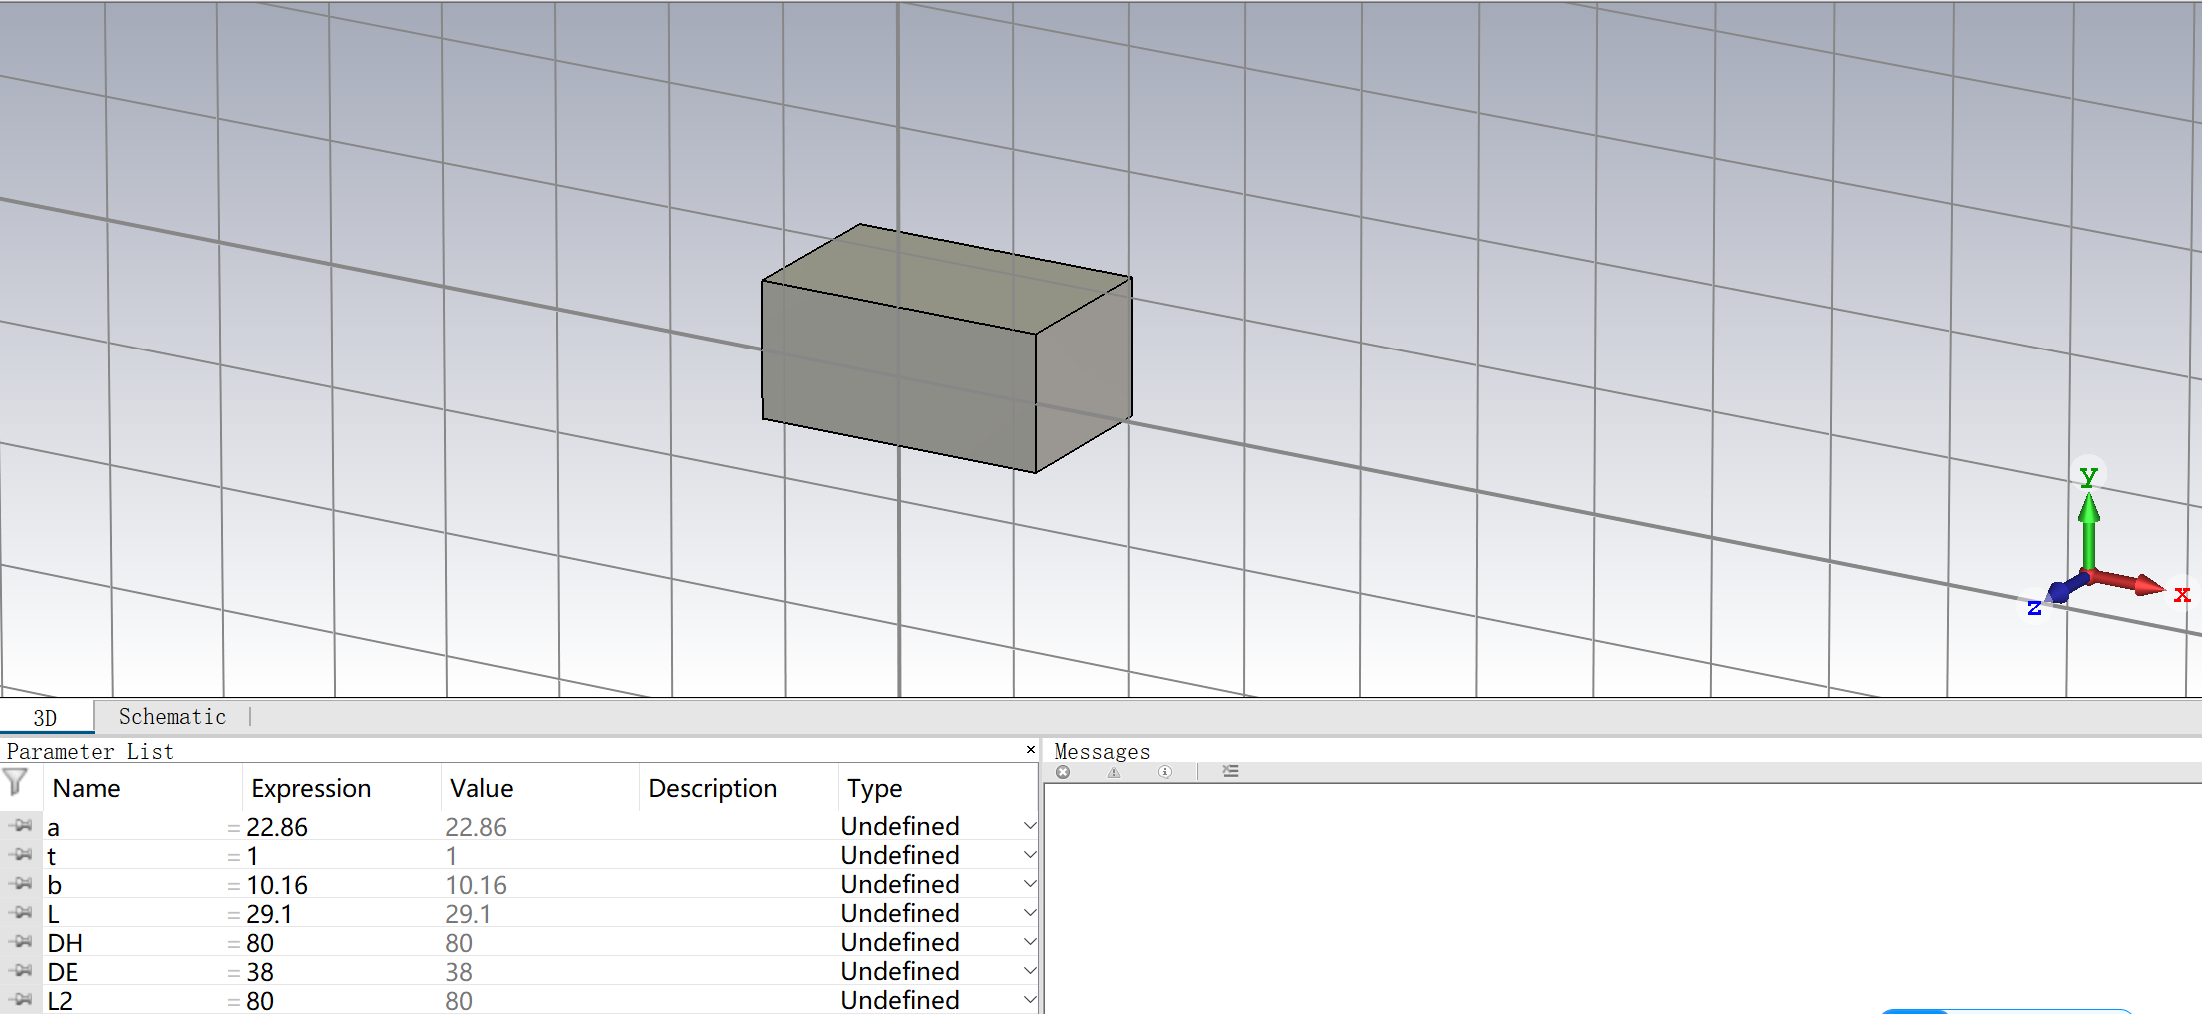
\includegraphics[width=0.65\linewidth]{figures/m1.png} % 数字表示放缩比例
			\caption{矩形波导模型图} % 图片标题
		  \end{figure}
        \end{itemize}
        \item 创建喇叭模型：
        \begin{itemize}
            \item 喇叭口径面：\texttt{Modeling->Curves->Rectangle；Modeling->Curve Tools->Cover Planar Curve}（Figure 6）。
            \begin{figure}[H]
				\centering
				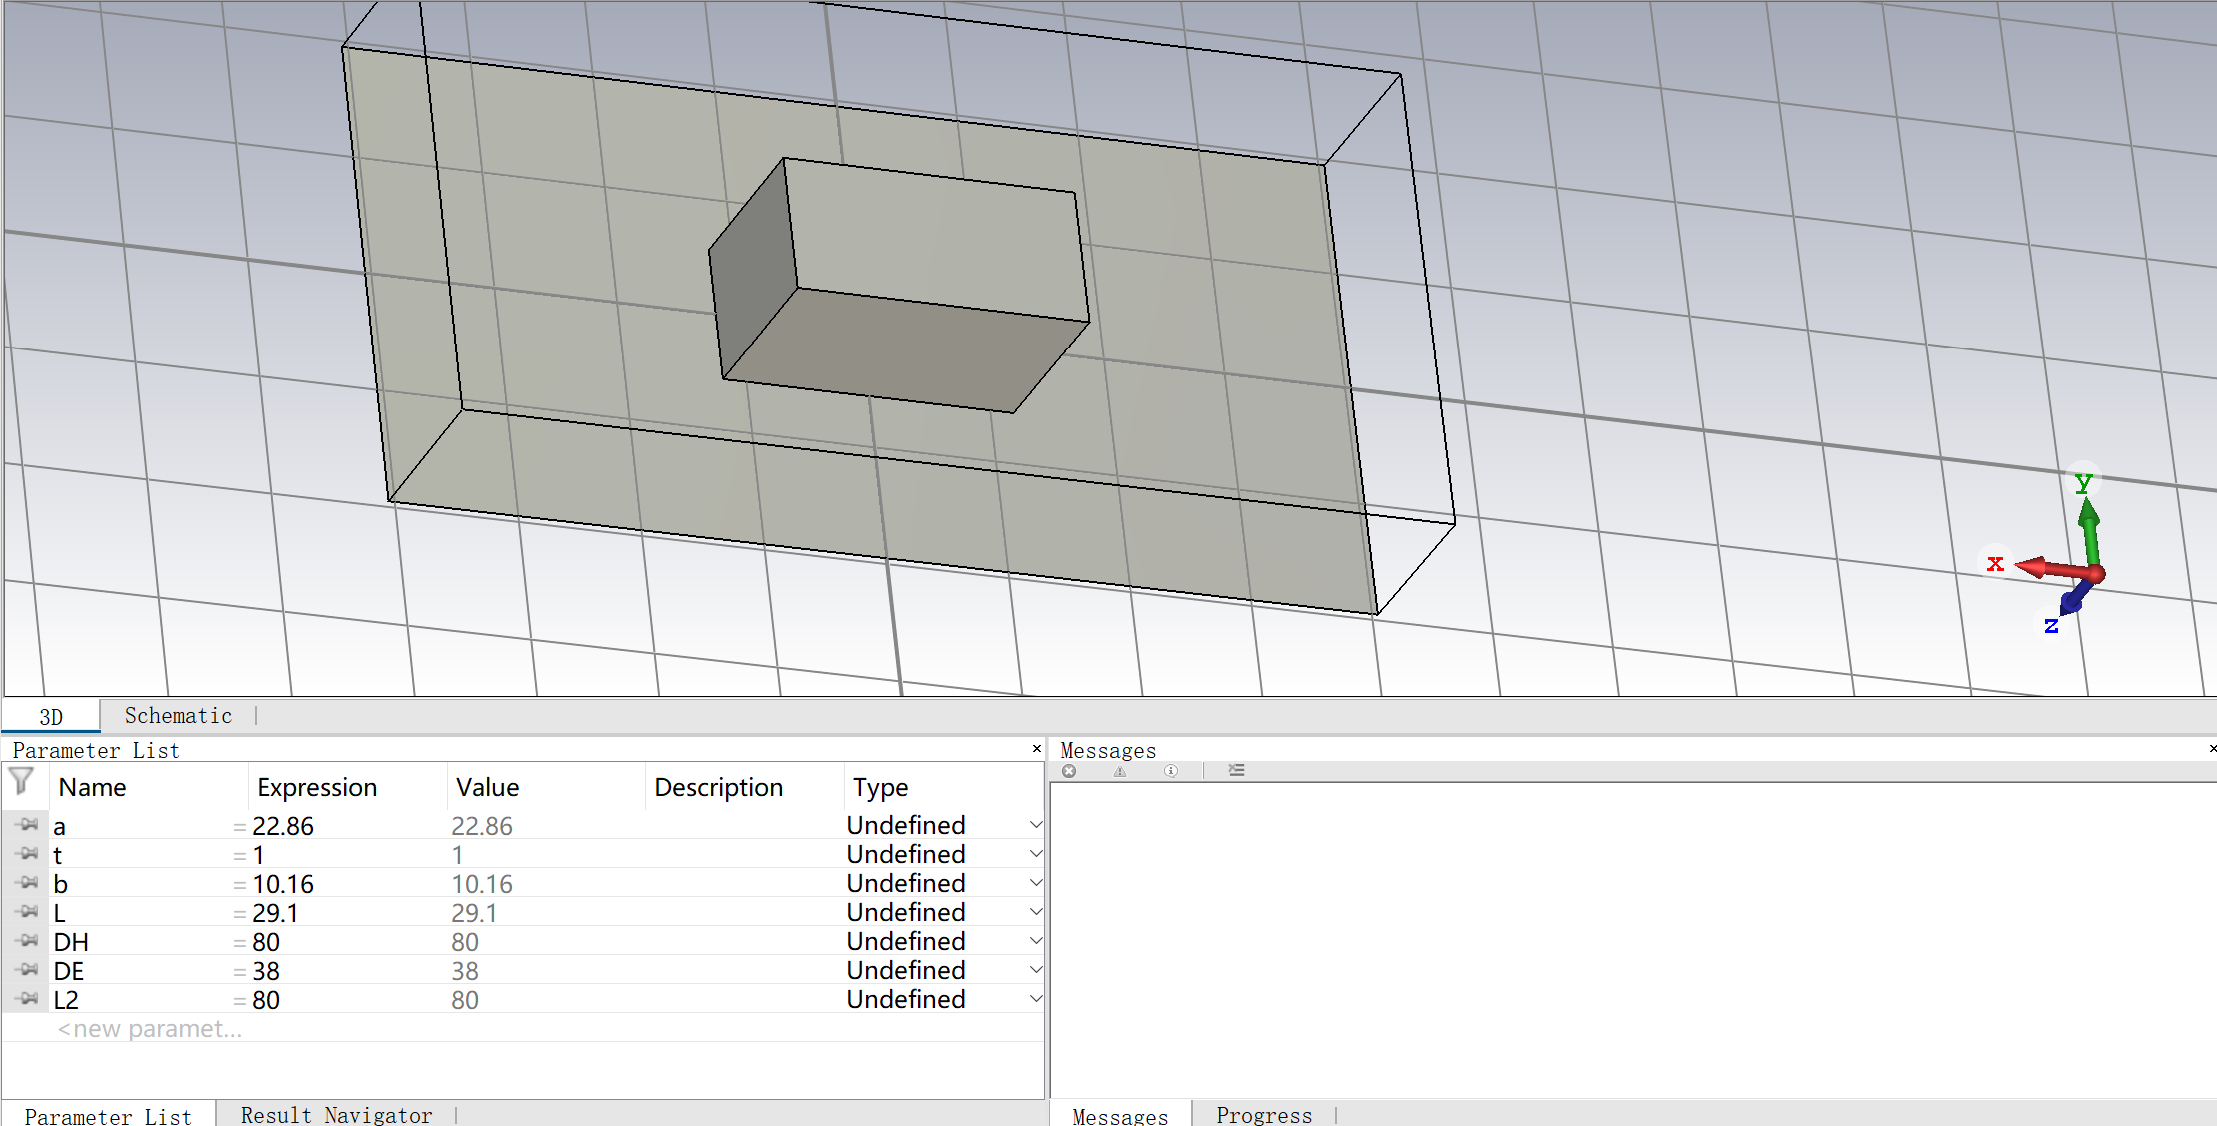
\includegraphics[width=0.65\linewidth]{figures/m2.png} % 数字表示放缩比例
				\caption{创建喇叭口径面} % 图片标题
			\end{figure}
            \item 设置口径面位置：\texttt{Modeling->Transform->Translate}（Figure 7）。
            \begin{figure}[H]
				\centering
				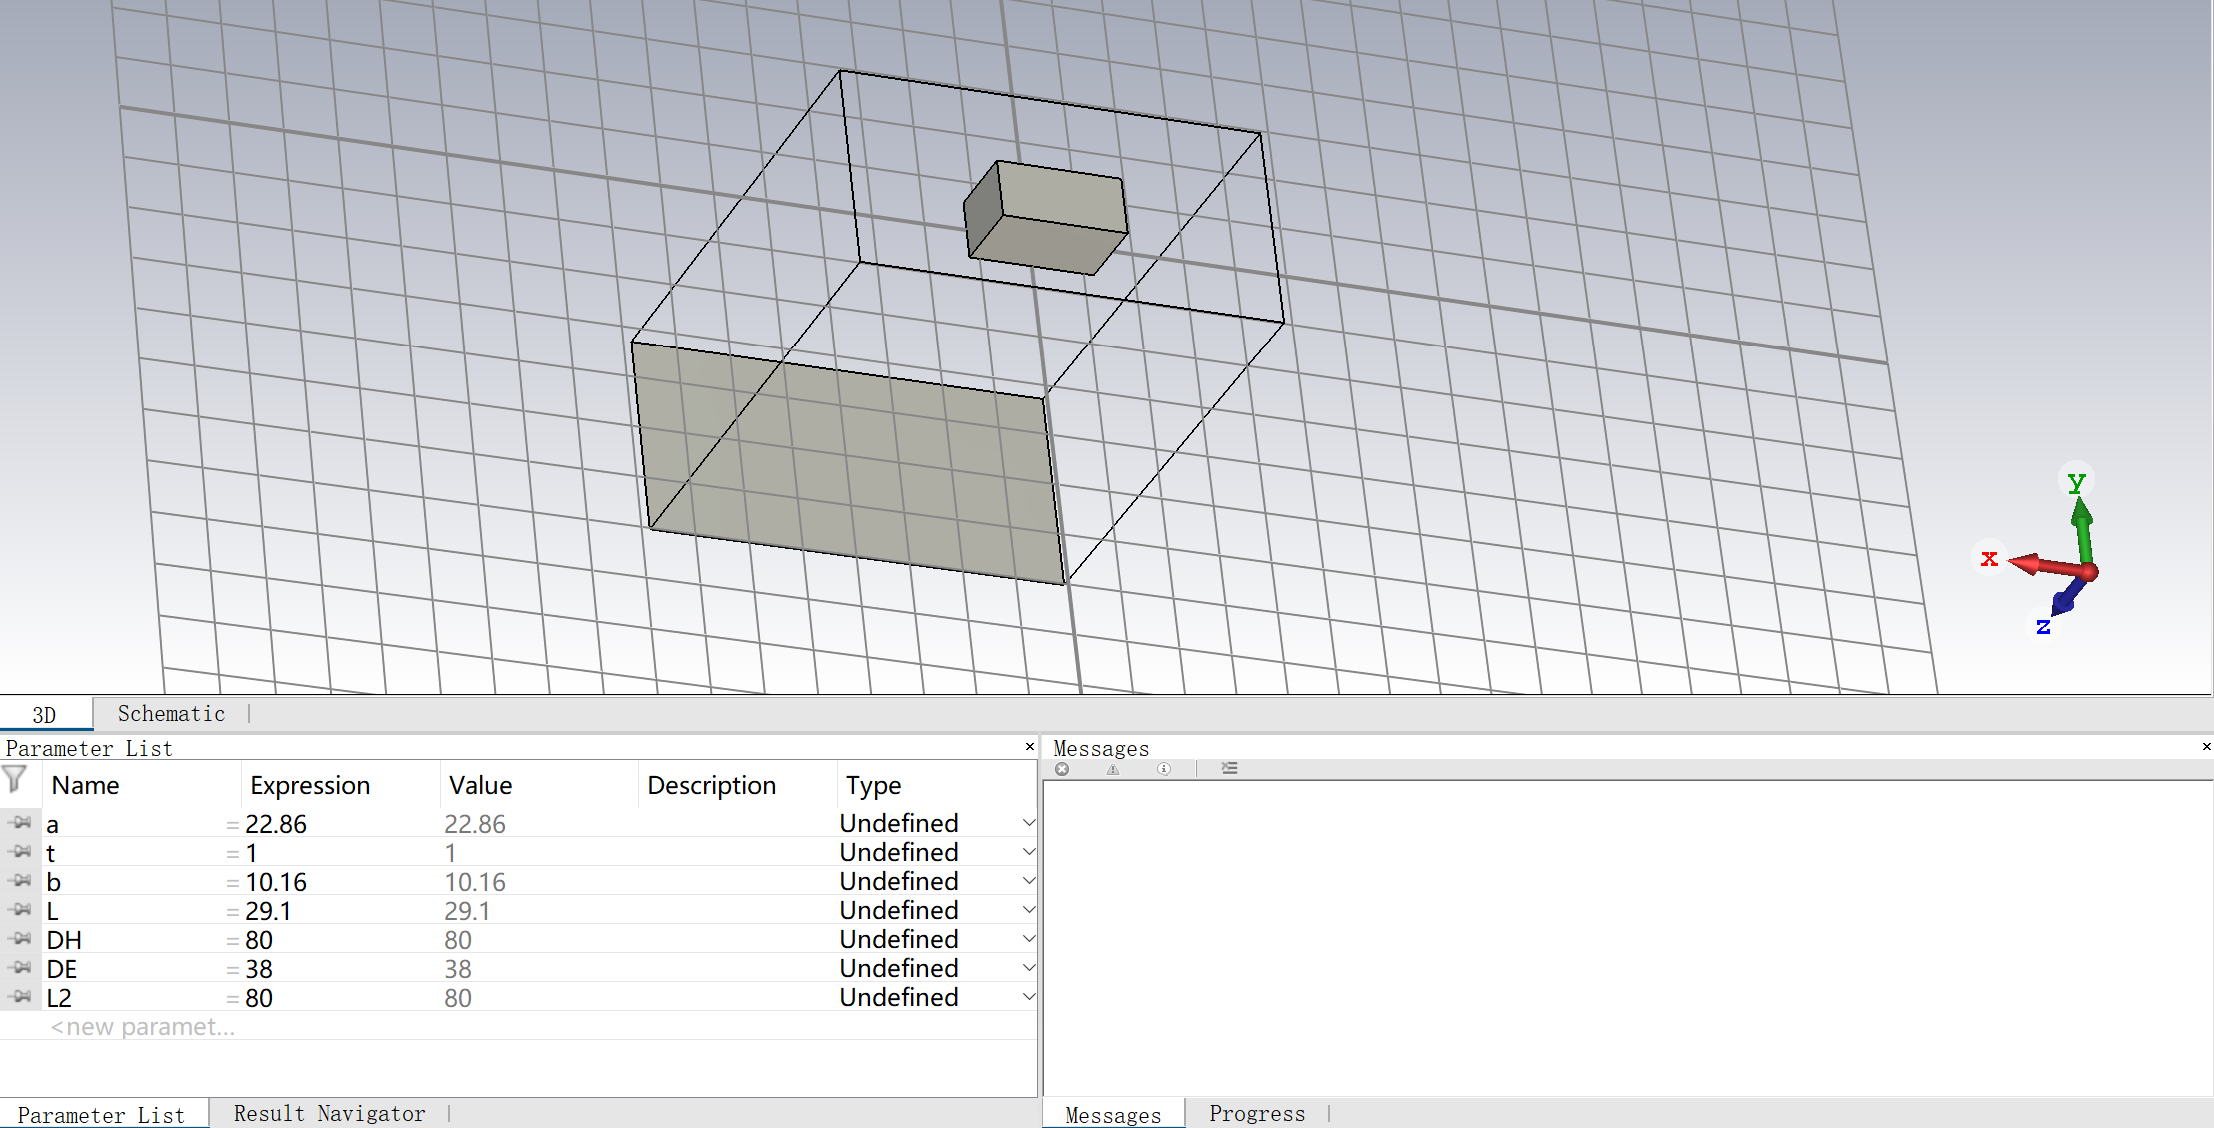
\includegraphics[width=0.65\linewidth]{figures/m3.png} % 数字表示放缩比例
				\caption{设置口径面位置} % 图片标题
			\end{figure}
			\item 创建侧壁：\texttt{Modeling->Shapes->Loft}（Figure 8）。
            \begin{figure}[H]
				\centering
				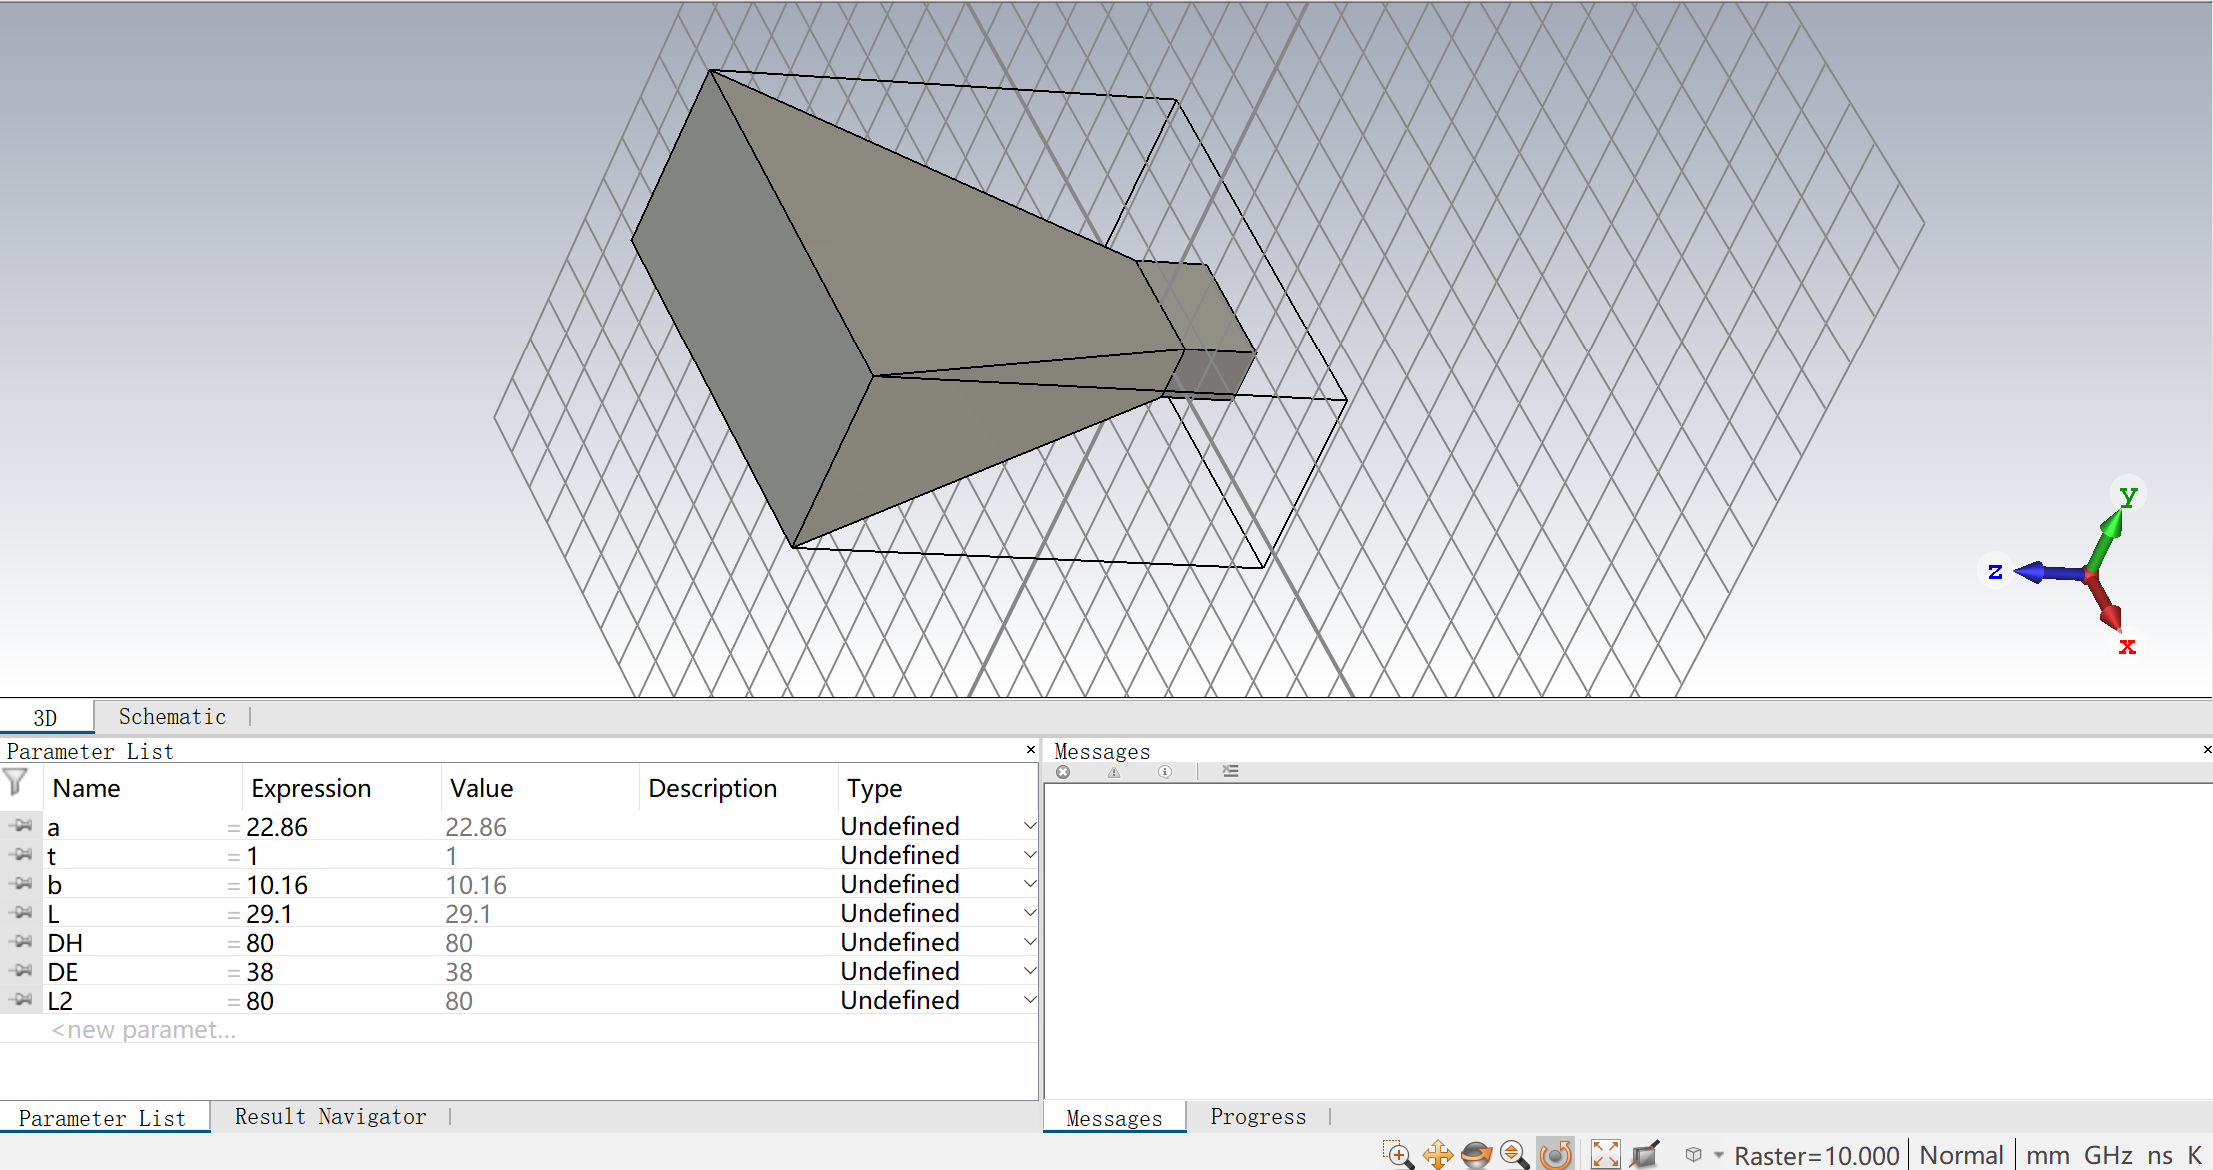
\includegraphics[width=0.65\linewidth]{figures/m4.png} % 数字表示放缩比例
				\caption{创建侧壁} % 图片标题
			\end{figure}
			\item 布尔运算：\texttt{Modeling->Boolean->Add} 合并物体。
			\begin{figure}[H]
				\centering
				\begin{minipage}[b]{0.5\linewidth}
					\centering
					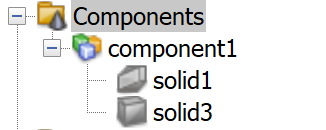
\includegraphics[width=0.9\textwidth]{figures/m5.png}
					\caption{布尔合并前}
				\end{minipage}%
				\begin{minipage}[b]{0.5\linewidth}
					\centering
					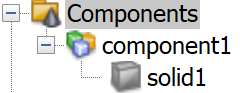
\includegraphics[width=0.9\textwidth]{figures/m6.png}
					\caption{布尔合并后}
				\end{minipage}
			  \end{figure}
		\end{itemize}
		\item 掏空: 
		\begin{itemize}
			\item 选择面：分别选取物体前后两个面
			\item 掏空生成喇叭：Modeling->Shapetools->Shell Solid or Thicken Sheet；
			\item 完成整个天线的CST建模，如Figure 11所示。
			\begin{figure}[H]
				\centering
				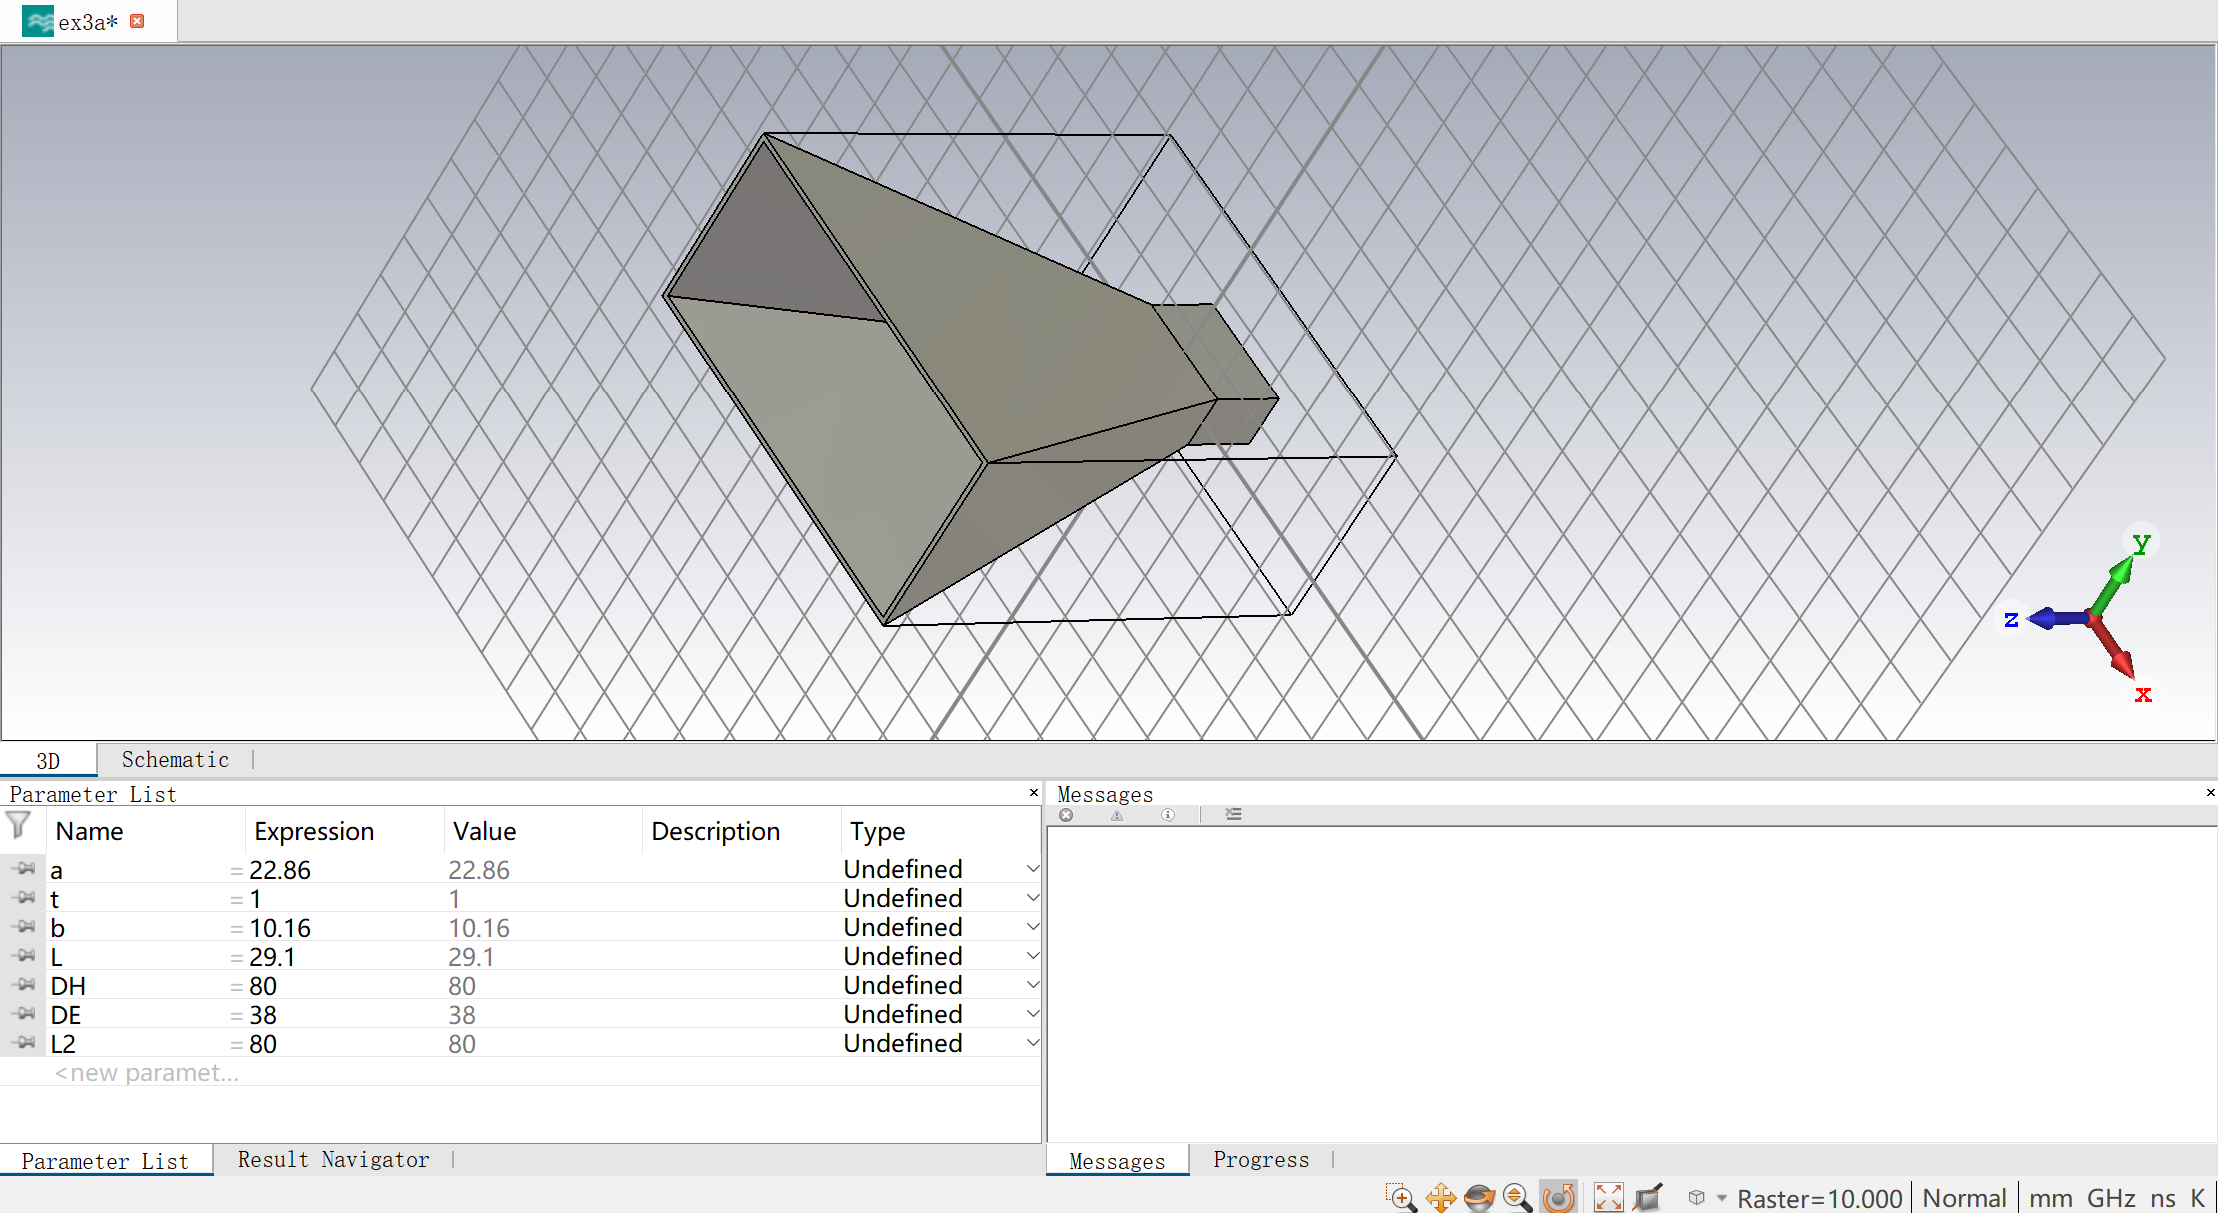
\includegraphics[width=0.65\linewidth]{figures/m7.png} % 数字表示放缩比例
				\caption{掏空后模型} % 图片标题
			\end{figure}
		\end{itemize}
    \end{enumerate}
    
    \item \textbf{设置仿真条件}
    \begin{enumerate}
        \item 频率范围：\texttt{Simulation->Frequency}（8.2GHz-12.4GHz）。
		\item 边界条件：\texttt{Simulation->Background->Normal；Simulation->Boundaries->open (add space)}。
        \begin{figure}[H]
			\centering
			\begin{minipage}[b]{0.5\linewidth}
				\centering
				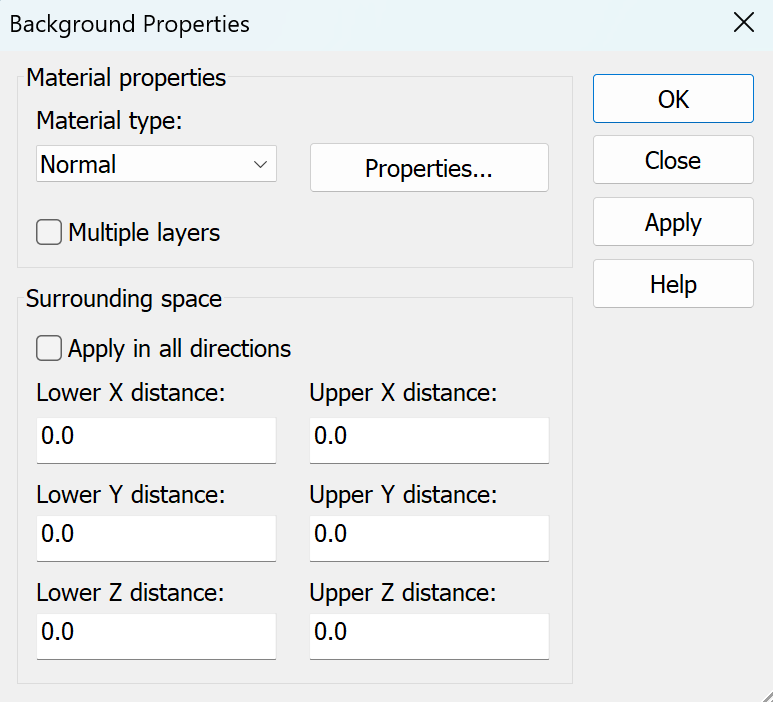
\includegraphics[width=0.9\textwidth]{figures/s2.png}
				\caption{背景条件}
			\end{minipage}%
			\begin{minipage}[b]{0.5\linewidth}
				\centering
				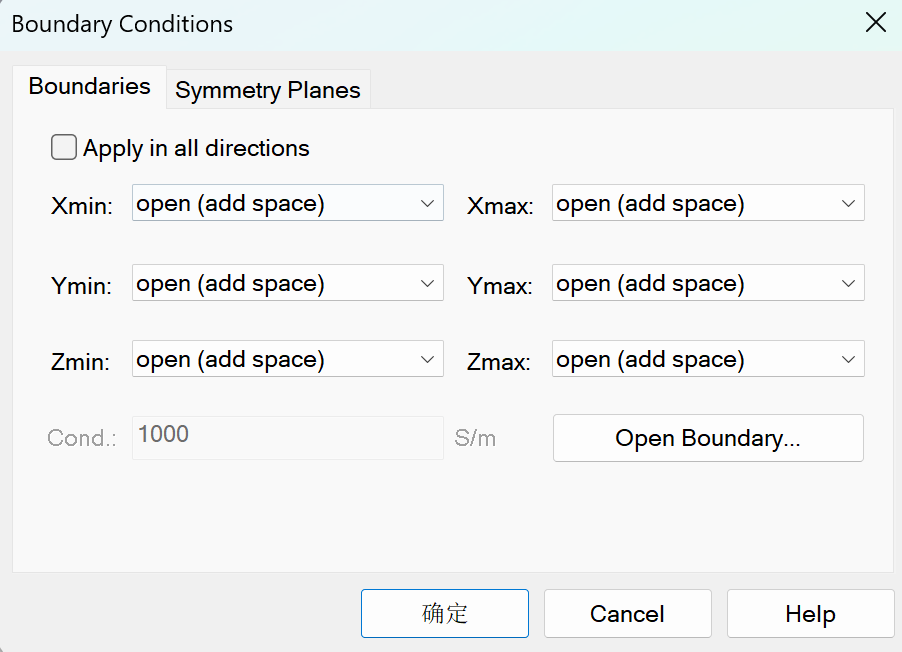
\includegraphics[width=0.9\textwidth]{figures/s3.png}
				\caption{边界条件}
			\end{minipage}
		  \end{figure}
		\item 端口设置：选取波导口面，设置 \texttt{Waveguide Port}，模式数设为5。
        \begin{figure}[H]
			\centering
			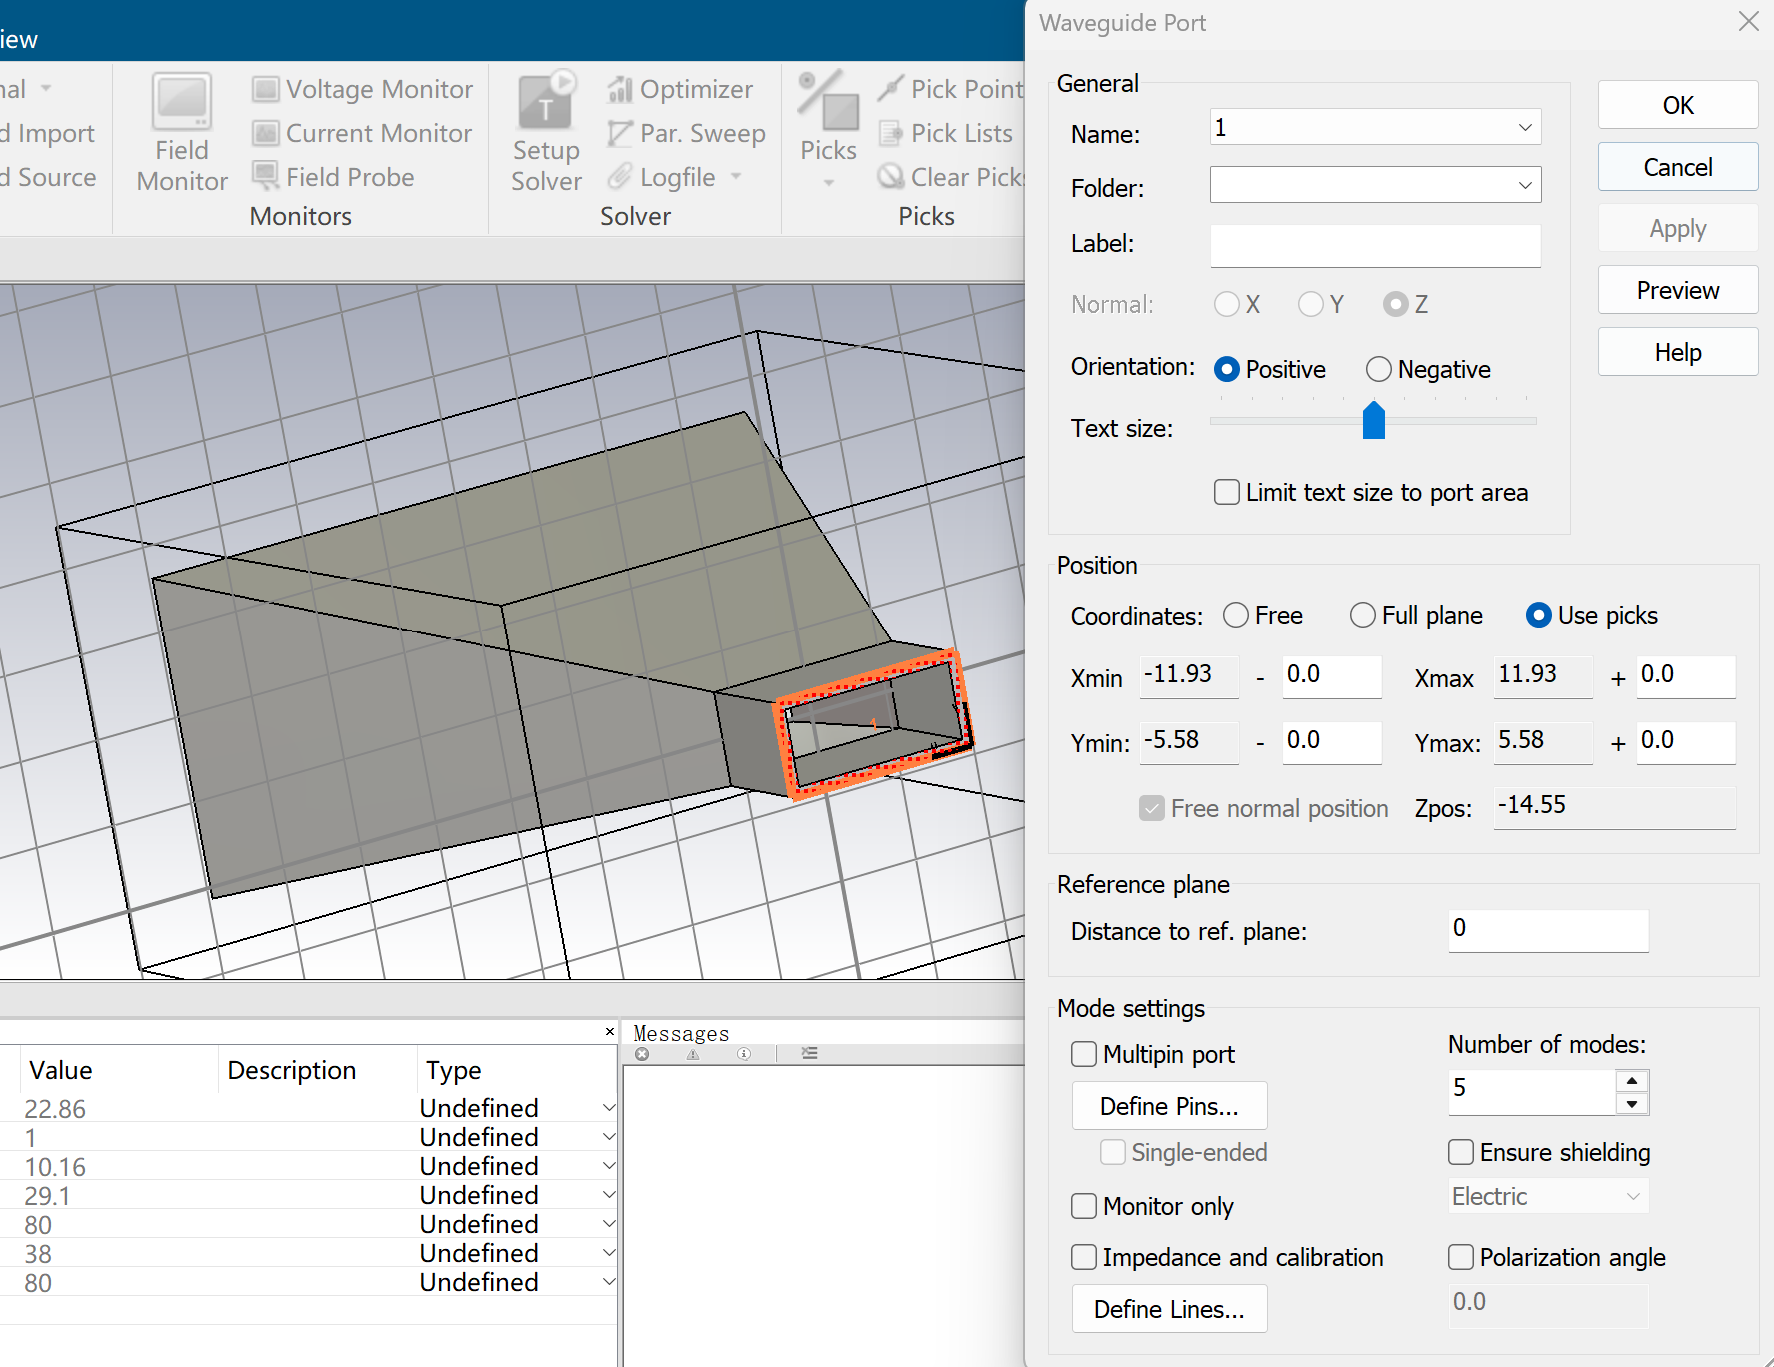
\includegraphics[width=0.65\linewidth]{figures/s4.png} % 数字表示放缩比例
			\caption{端口设置} % 图片标题
		\end{figure}
		\item 监视器：设置远场监视器（10.3GHz），\texttt{Simulation->Field Monitor->Farfield（RCS）}。
		\begin{figure}[H]
			\centering
			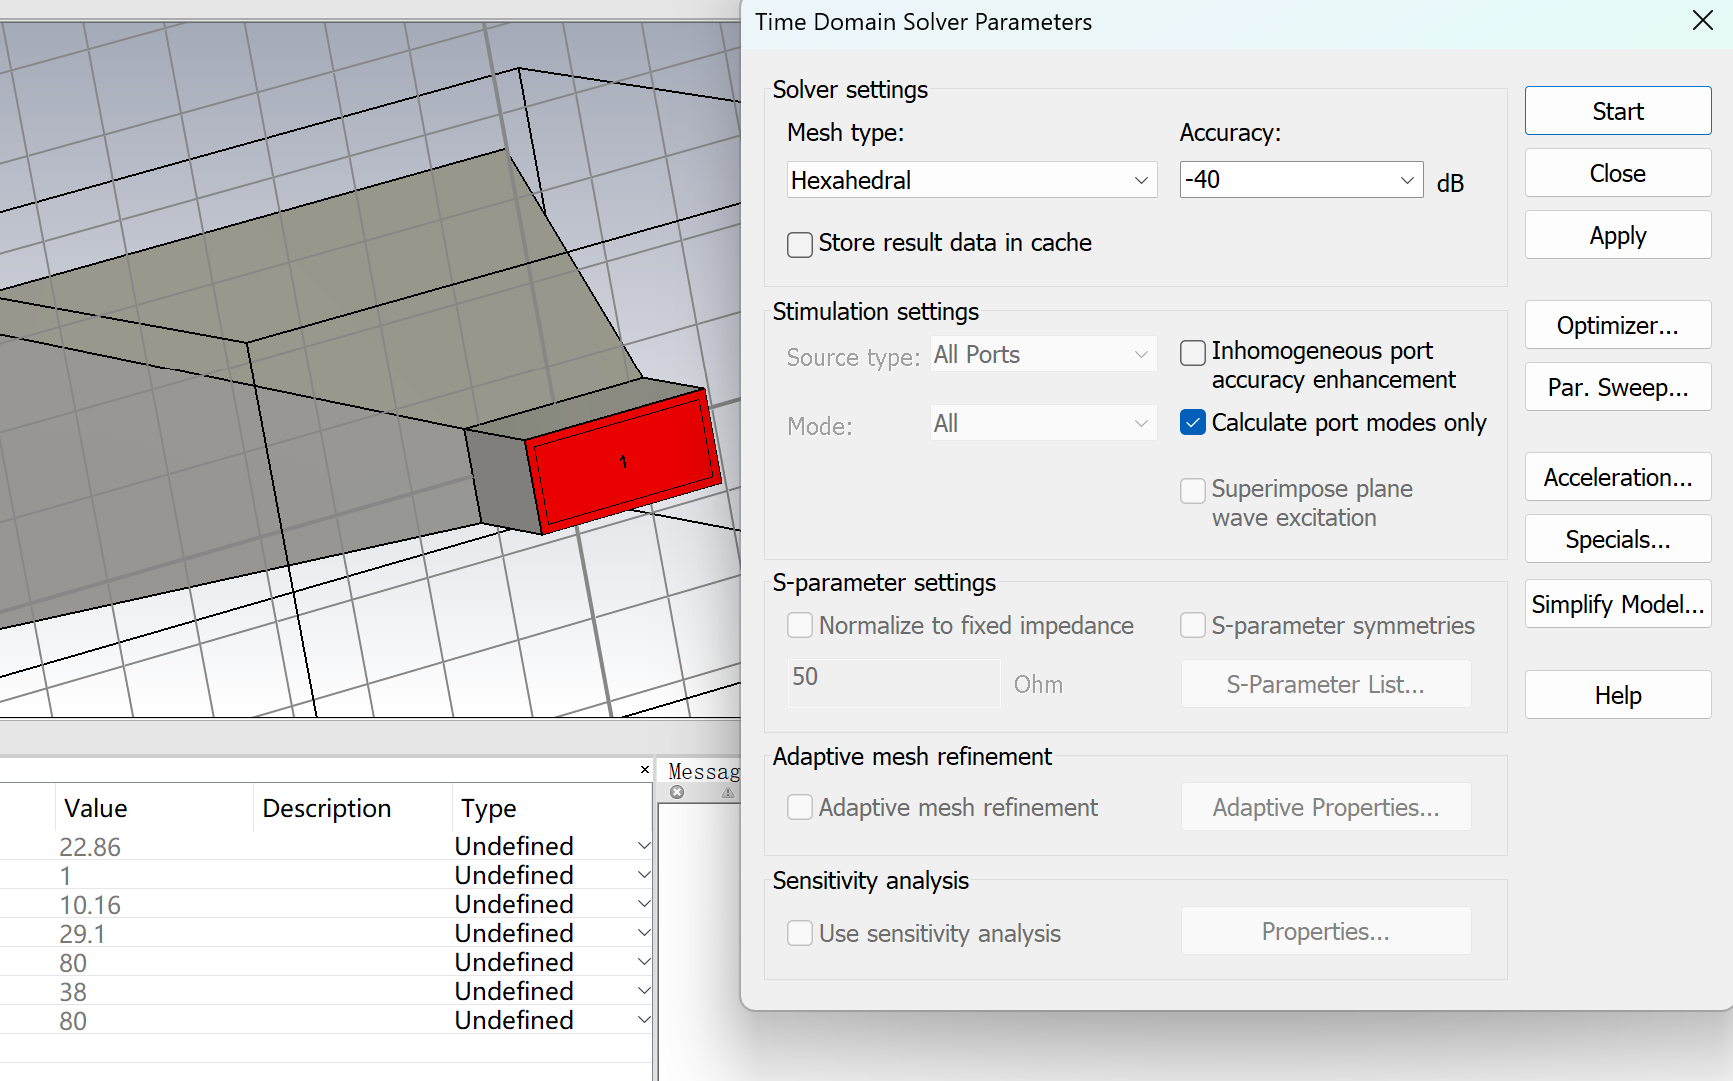
\includegraphics[width=0.65\linewidth]{figures/s5.png} % 数字表示放缩比例
			\caption{监视器设置} % 图片标题
		\end{figure}
	\end{enumerate}
\end{enumerate}

\subsection{模式分析}
\begin{enumerate}
    \item \textbf{模式分析设置}\\
    \texttt{Simulation->Start Simulation->Source type: All Ports Modes: All}，勾选 \texttt{Calculate modes only}。
    \begin{figure}[H]
		\centering
		\begin{minipage}[b]{0.5\linewidth}
			\centering
			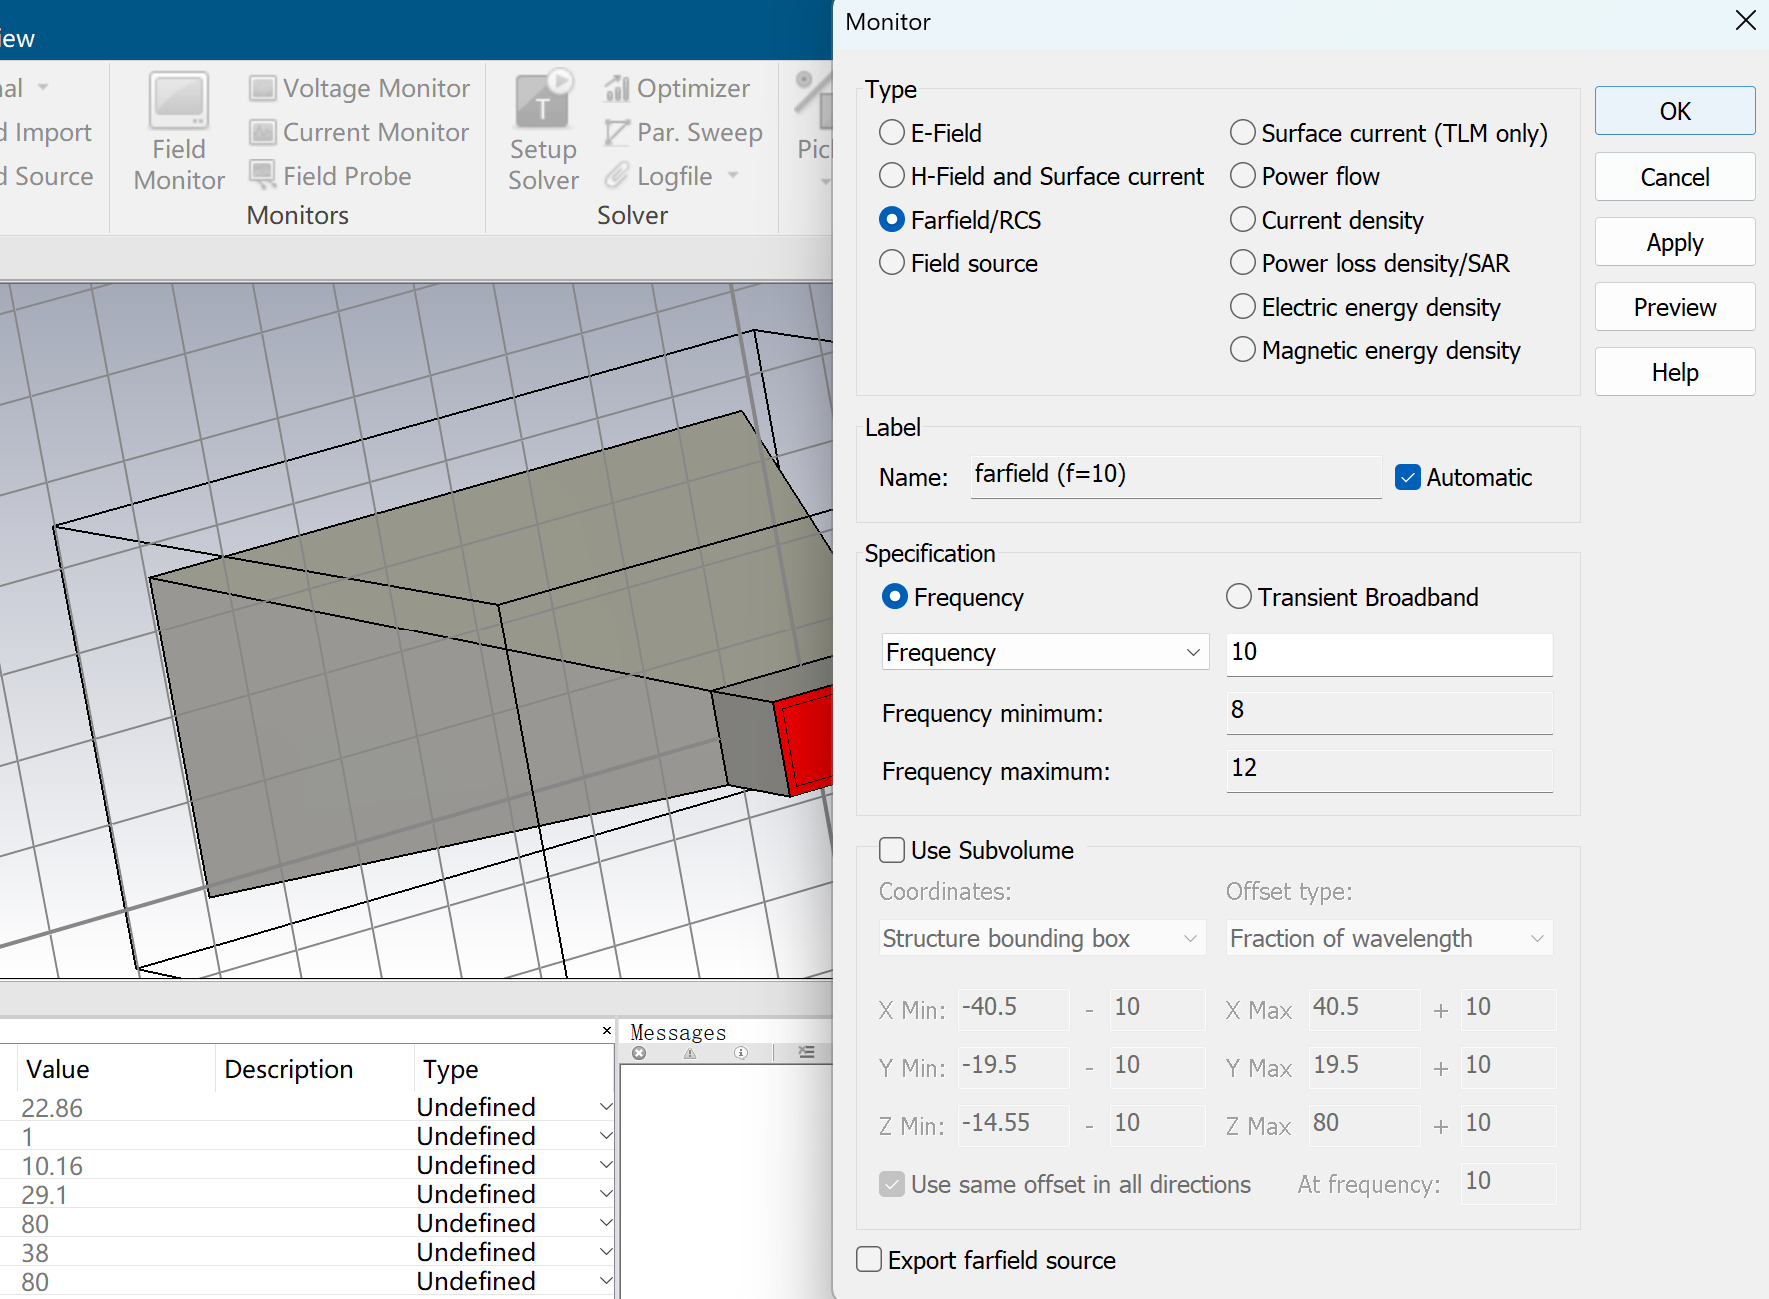
\includegraphics[width=0.9\textwidth]{figures/s6.png}
			\caption{模式分析}
		\end{minipage}%
		\begin{minipage}[b]{0.5\linewidth}
			\centering
			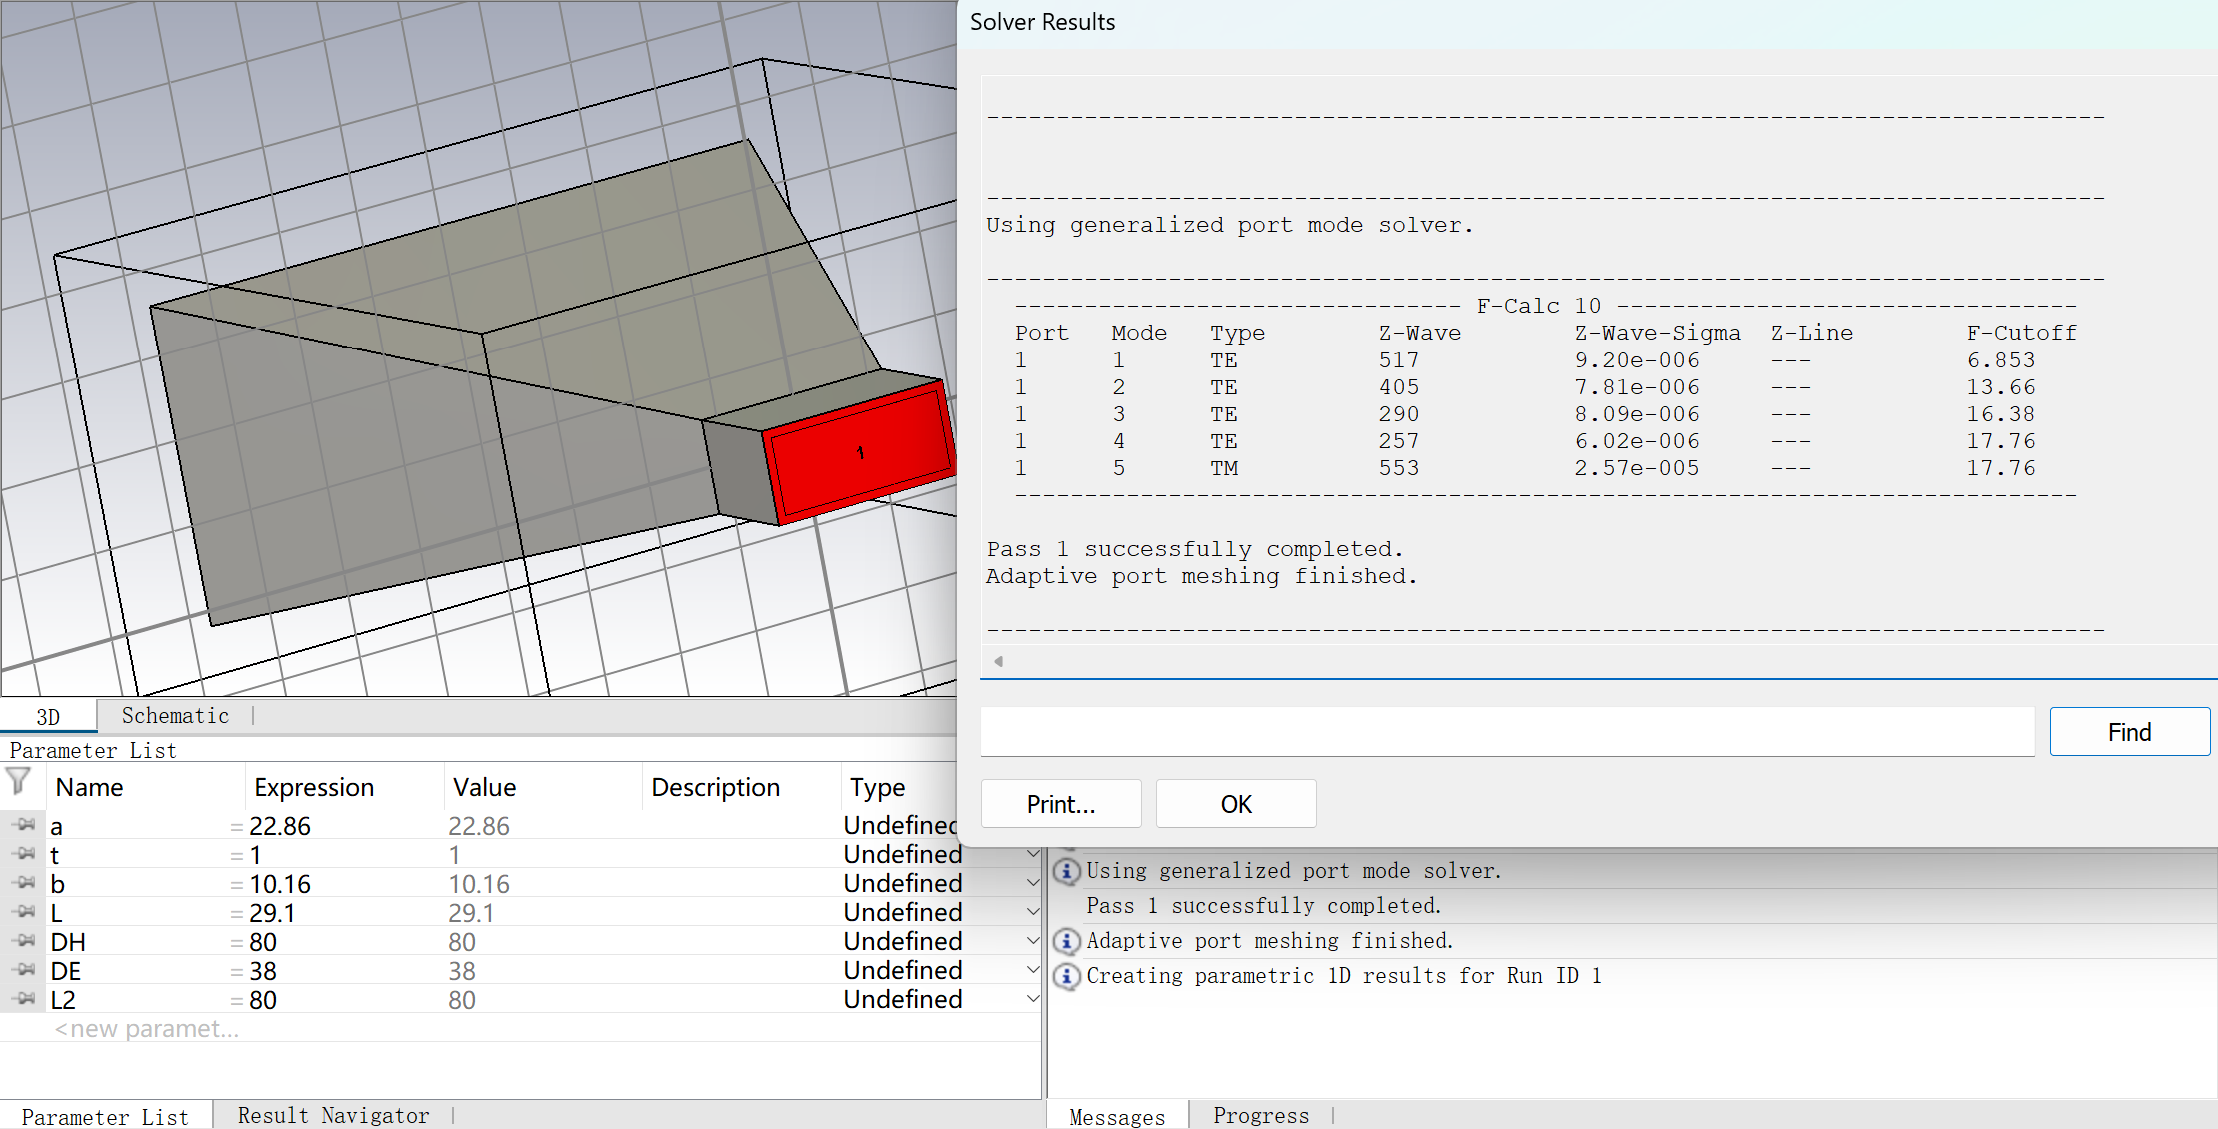
\includegraphics[width=0.9\textwidth]{figures/s7.png}
			\caption{模式分析结果}
		\end{minipage}
	  \end{figure}

	\item \textbf{模式仿真分析}\\
    仿真日志显示仅传输1种模式（图4-27），模式数设置大于1即可。
	\begin{figure}[H]
		\centering
		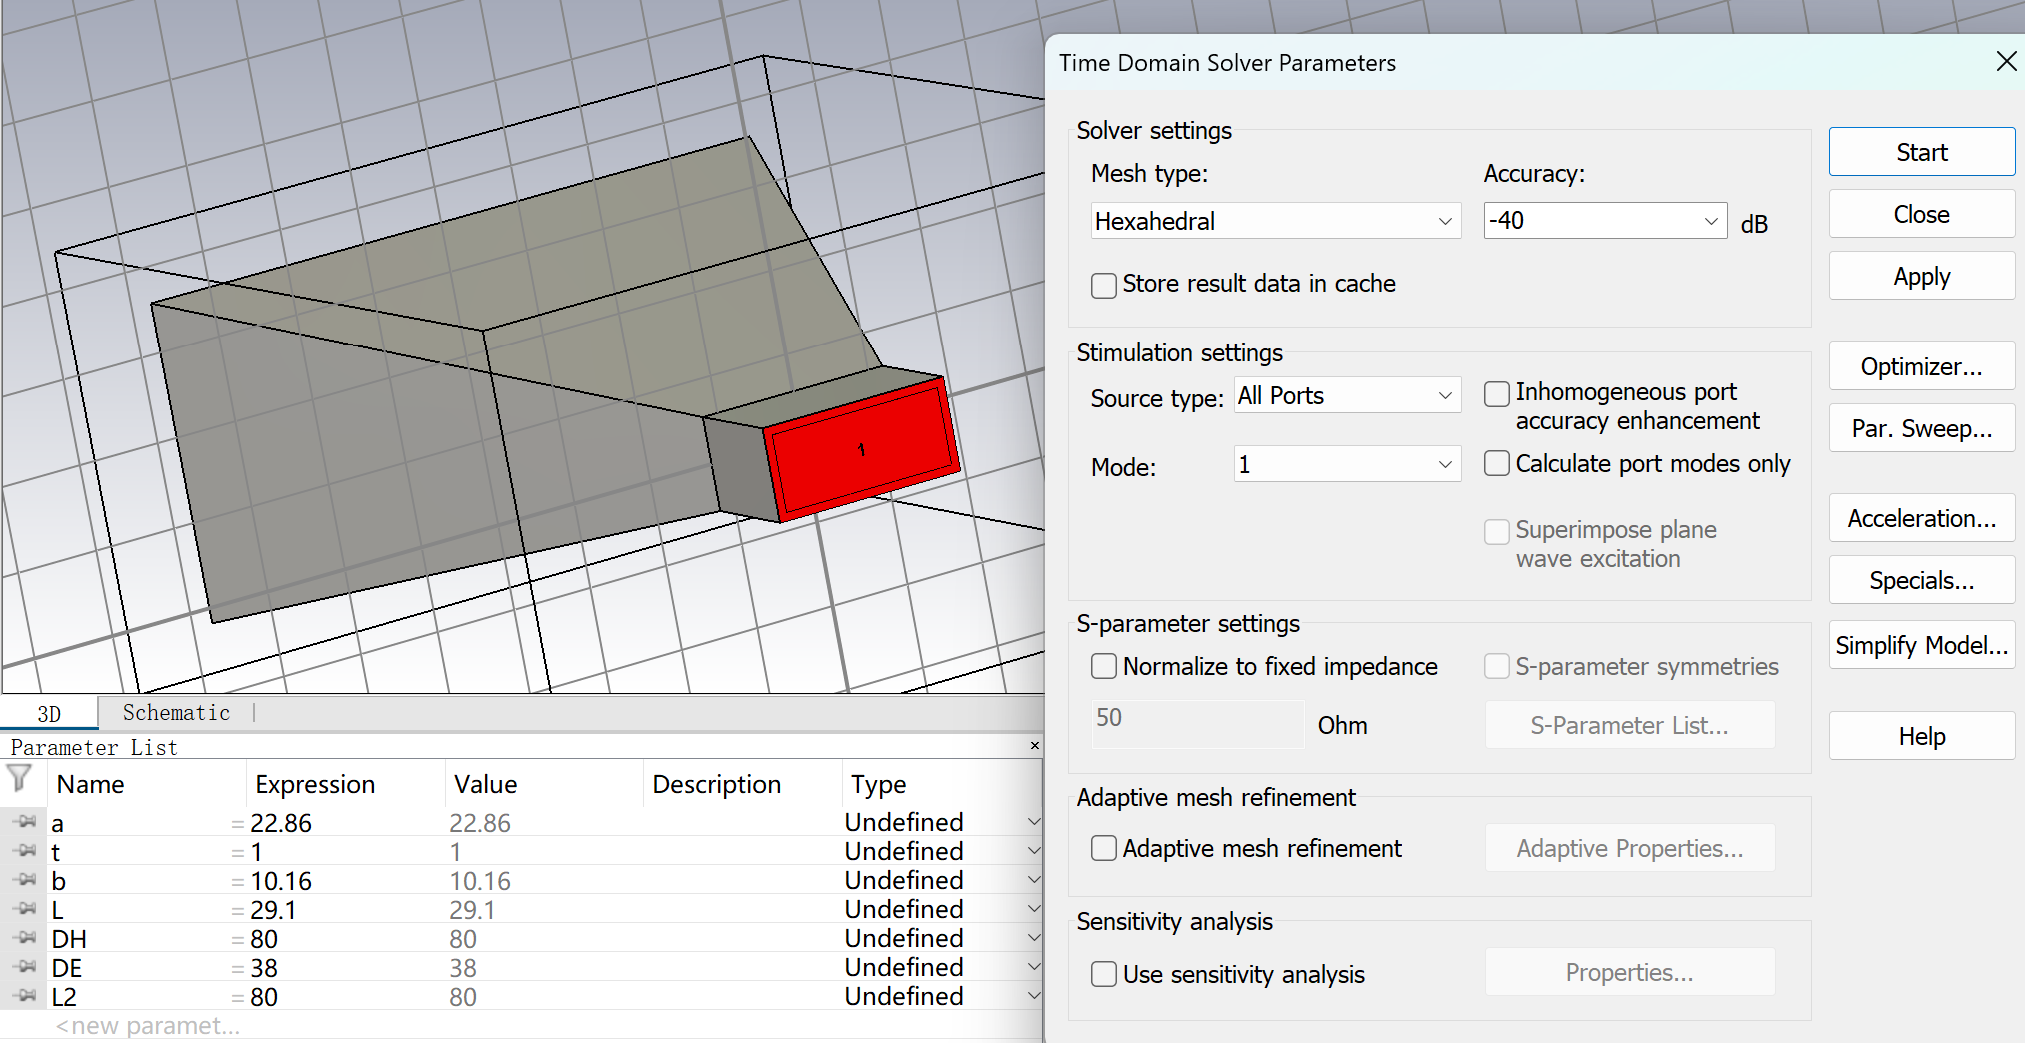
\includegraphics[width=0.65\linewidth]{figures/s8.png} % 数字表示放缩比例
		\caption{开始仿真} % 图片标题
	\end{figure}
	\item \textbf{电场、磁场、表面电流仿真}\\
    仿真结束后，在 Field Monitor 中选择 E-Field，增加电场仿真，同理再次选择H-Field and surface current，增加磁场和表面电流仿真仿真。
	\begin{figure}[H]
		\centering
		\includegraphics[width=0.65\linewidth]{figures/s9.png} % 数字表示放缩比例
		\caption{电场、磁场、表面电流仿真} % 图片标题
	\end{figure}
\end{enumerate}
\clearpage

\section{仿真结果图和曲线}
\subsection{分析喇叭天线S11和驻波比特性曲线}
\begin{figure}[H]
	\centering
	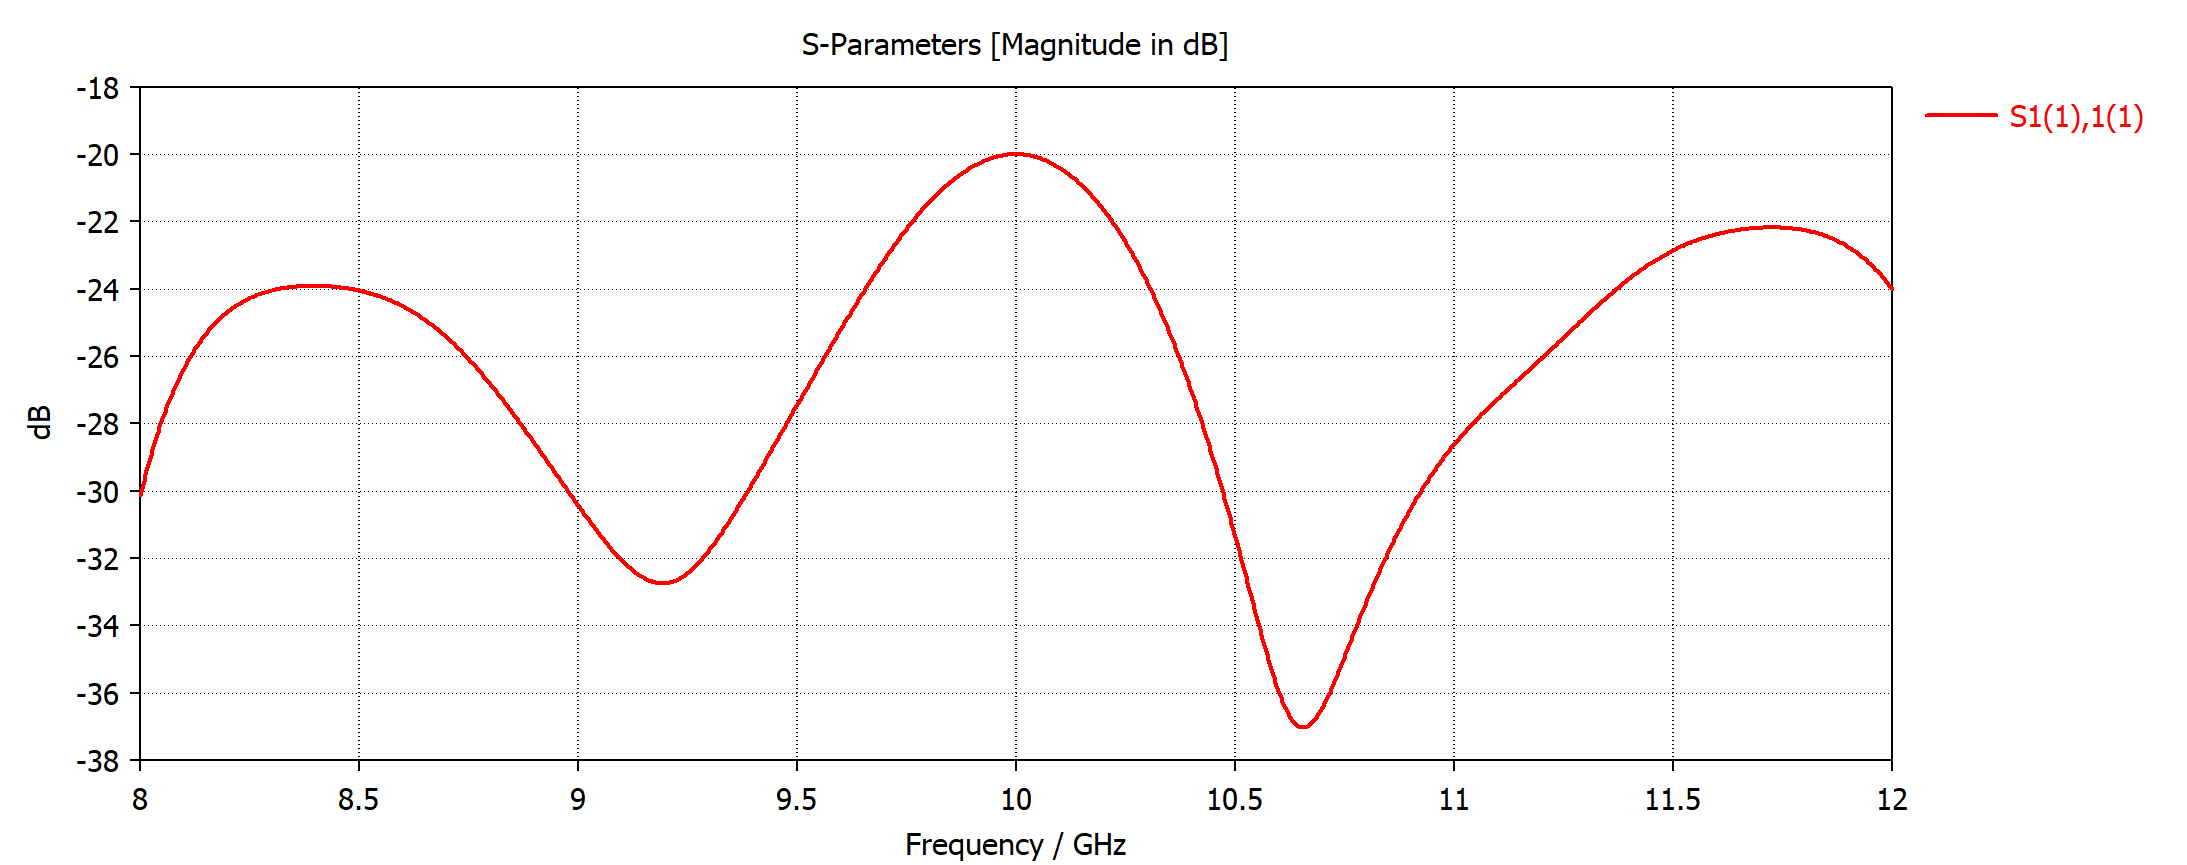
\includegraphics[width=0.65\linewidth]{figures/A11.png} % 数字表示放缩比例
	\caption{S11特性曲线} % 图片标题
\end{figure}
【分析】：S11表示端口反射信号与入射信号的比值，反映了天线的匹配情况。
从图中可以看出，S11在10.7 GHz左右达到了最低点，约为-37 dB，表示此频率下的反射信号最小，天线的匹配较好。随着频率的增高或减低，S11的幅度增大，反射信号增多，匹配变差。
整体曲线呈现出一定的波动，但总体而言，反射系数均在-20dB以下，工作特性良好，并在9.2GHz与10.7GHz附近工作时较优。
\begin{figure}[H]
	\centering
	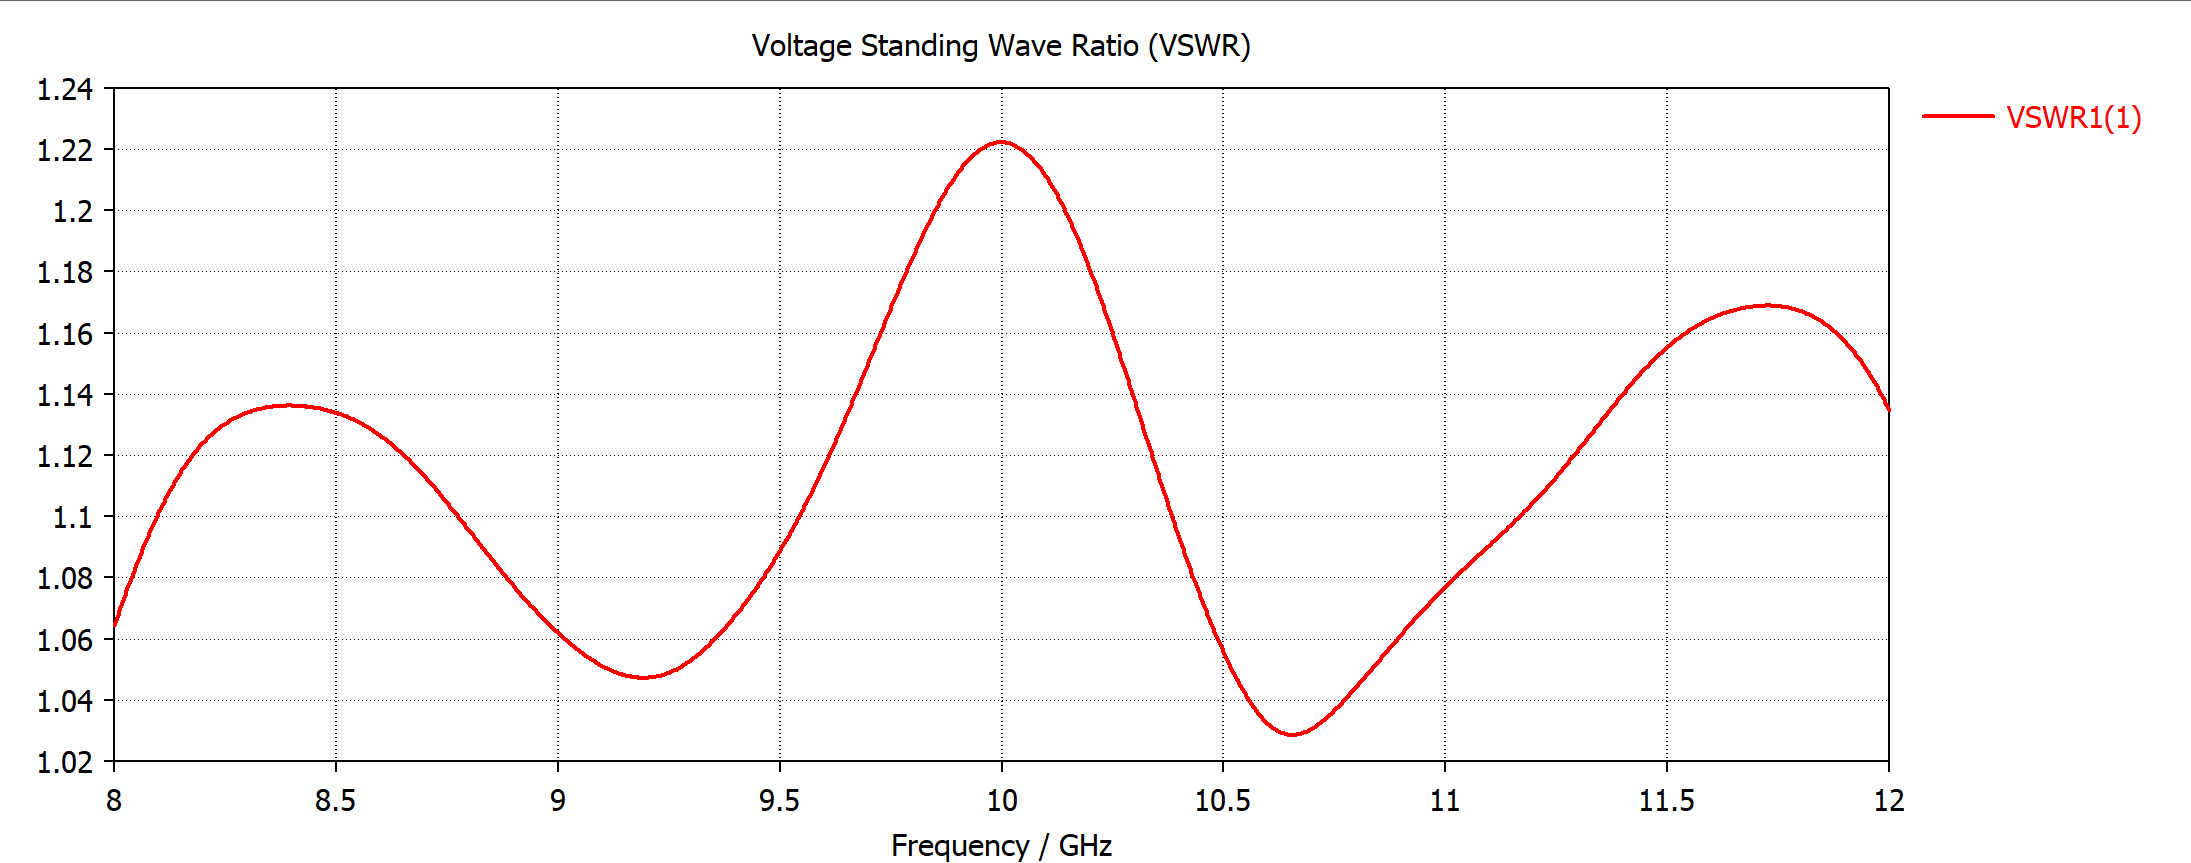
\includegraphics[width=0.65\linewidth]{figures/A12.png} % 数字表示放缩比例
	\caption{驻波比特性曲线} % 图片标题
\end{figure}
【分析】：驻波比能反映天线反射情况，驻波比越接近于1反射越小。
从图中可以看出，驻波比特性曲线整体特性与S11特性曲线相似，在10.7 GHz左右达到了最低点，约为1.03，表示此频率下的反射信号最小，天线的匹配较好。随着频率的增高或减低，
驻波比增大，反射信号增多，匹配变差。
整体曲线呈现出一定的波动，但总体而言，驻波比均在1.22以下，工作特性良好，并在9.2GHz与10.7GHz附近工作时较优。
\subsection{分析喇叭天线的水平、垂直方向图}

\begin{figure}[H]
	\centering
	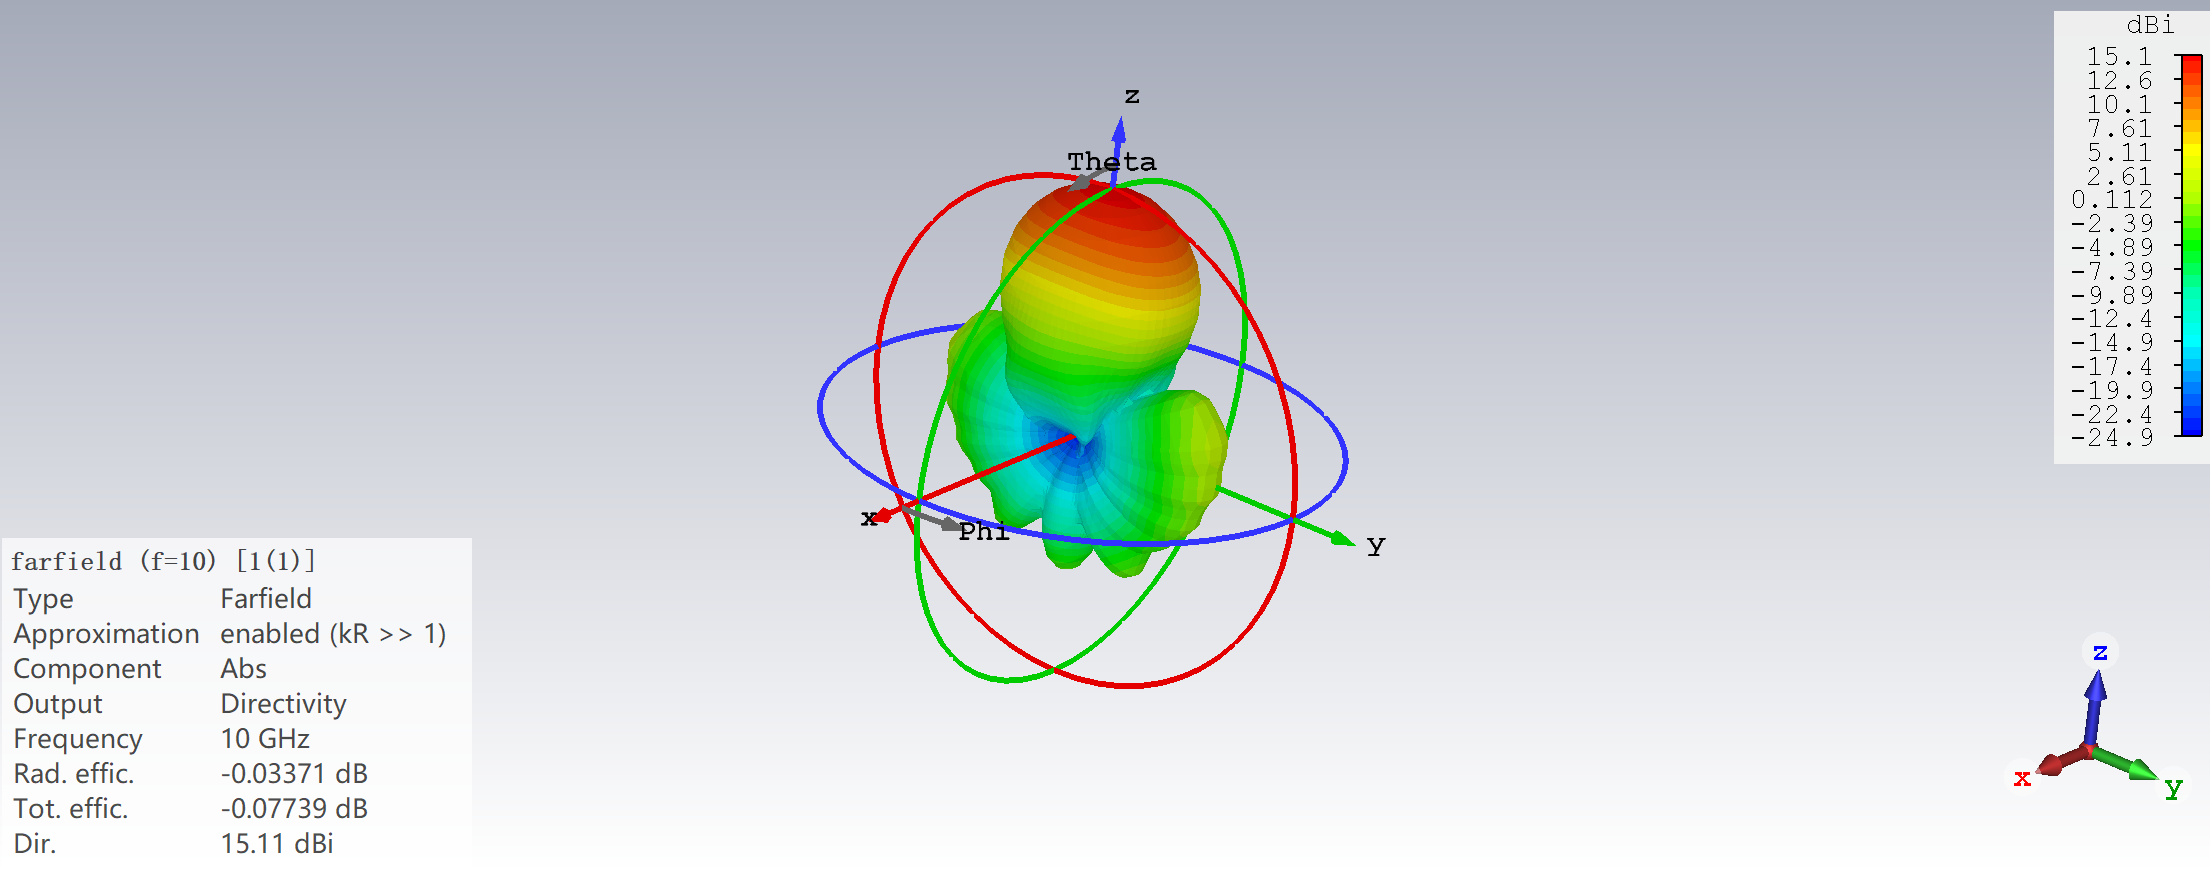
\includegraphics[width=0.65\linewidth]{figures/A21.png} % 数字表示放缩比例
	\caption{3D 仿真结果} % 图片标题
\end{figure}
【分析】：颜色标度显示了不同方向上的辐射强度。最高的辐射强度为15.1 dBi，出现z轴正方向上
\begin{figure}[H]
	\centering
	\begin{minipage}[b]{0.5\linewidth}
		\centering
		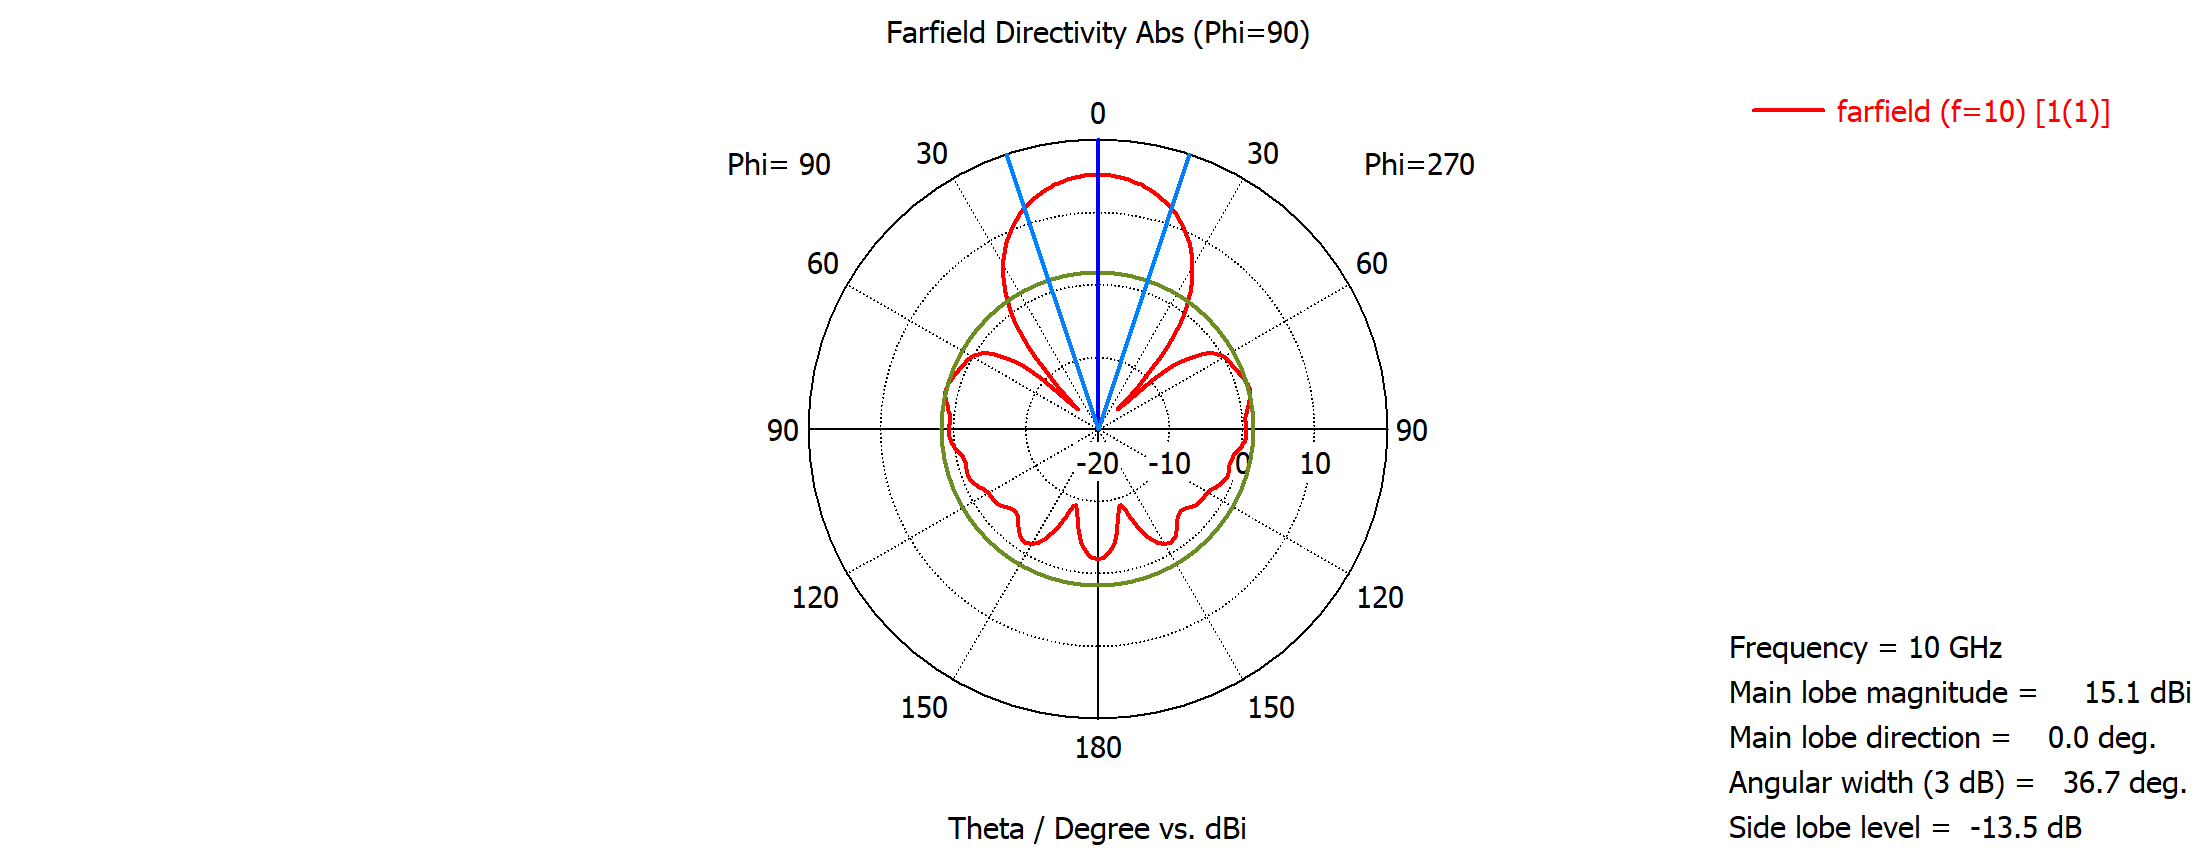
\includegraphics[width=1.0\textwidth]{figures/A22.png}
		\caption{$\phi = 90$方向图}
	\end{minipage}%
	\begin{minipage}[b]{0.5\linewidth}
		\centering
		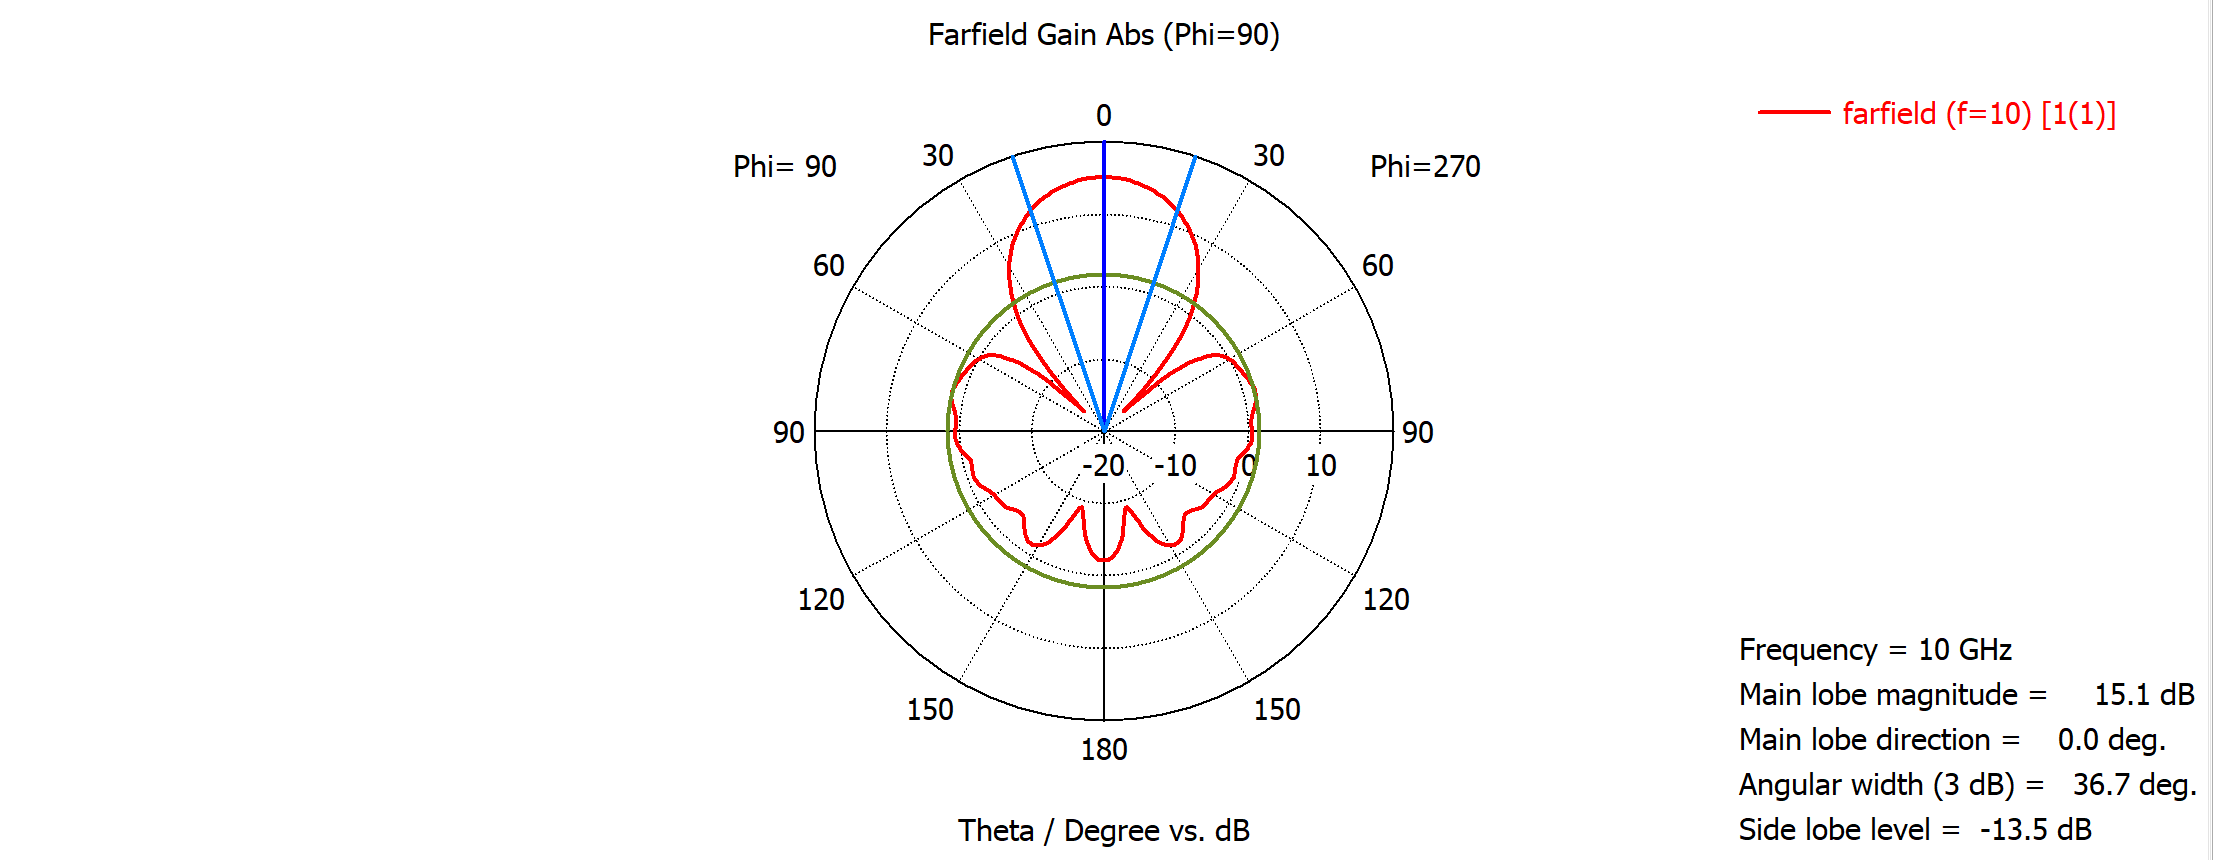
\includegraphics[width=1.0\textwidth]{figures/A22_.png}
		\caption{$\phi = 90$增益图}
	\end{minipage}
\end{figure}
【分析】：$\phi = 90$时，主瓣的方向为0度，最大辐射为15.1 dB。该图的3 dB角宽度为36.7度，副瓣为-13.5 dB，表示主瓣的方向性较强，而副瓣的辐射较小
\begin{figure}[H]
	\centering
	\begin{minipage}[b]{0.5\linewidth}
		\centering
		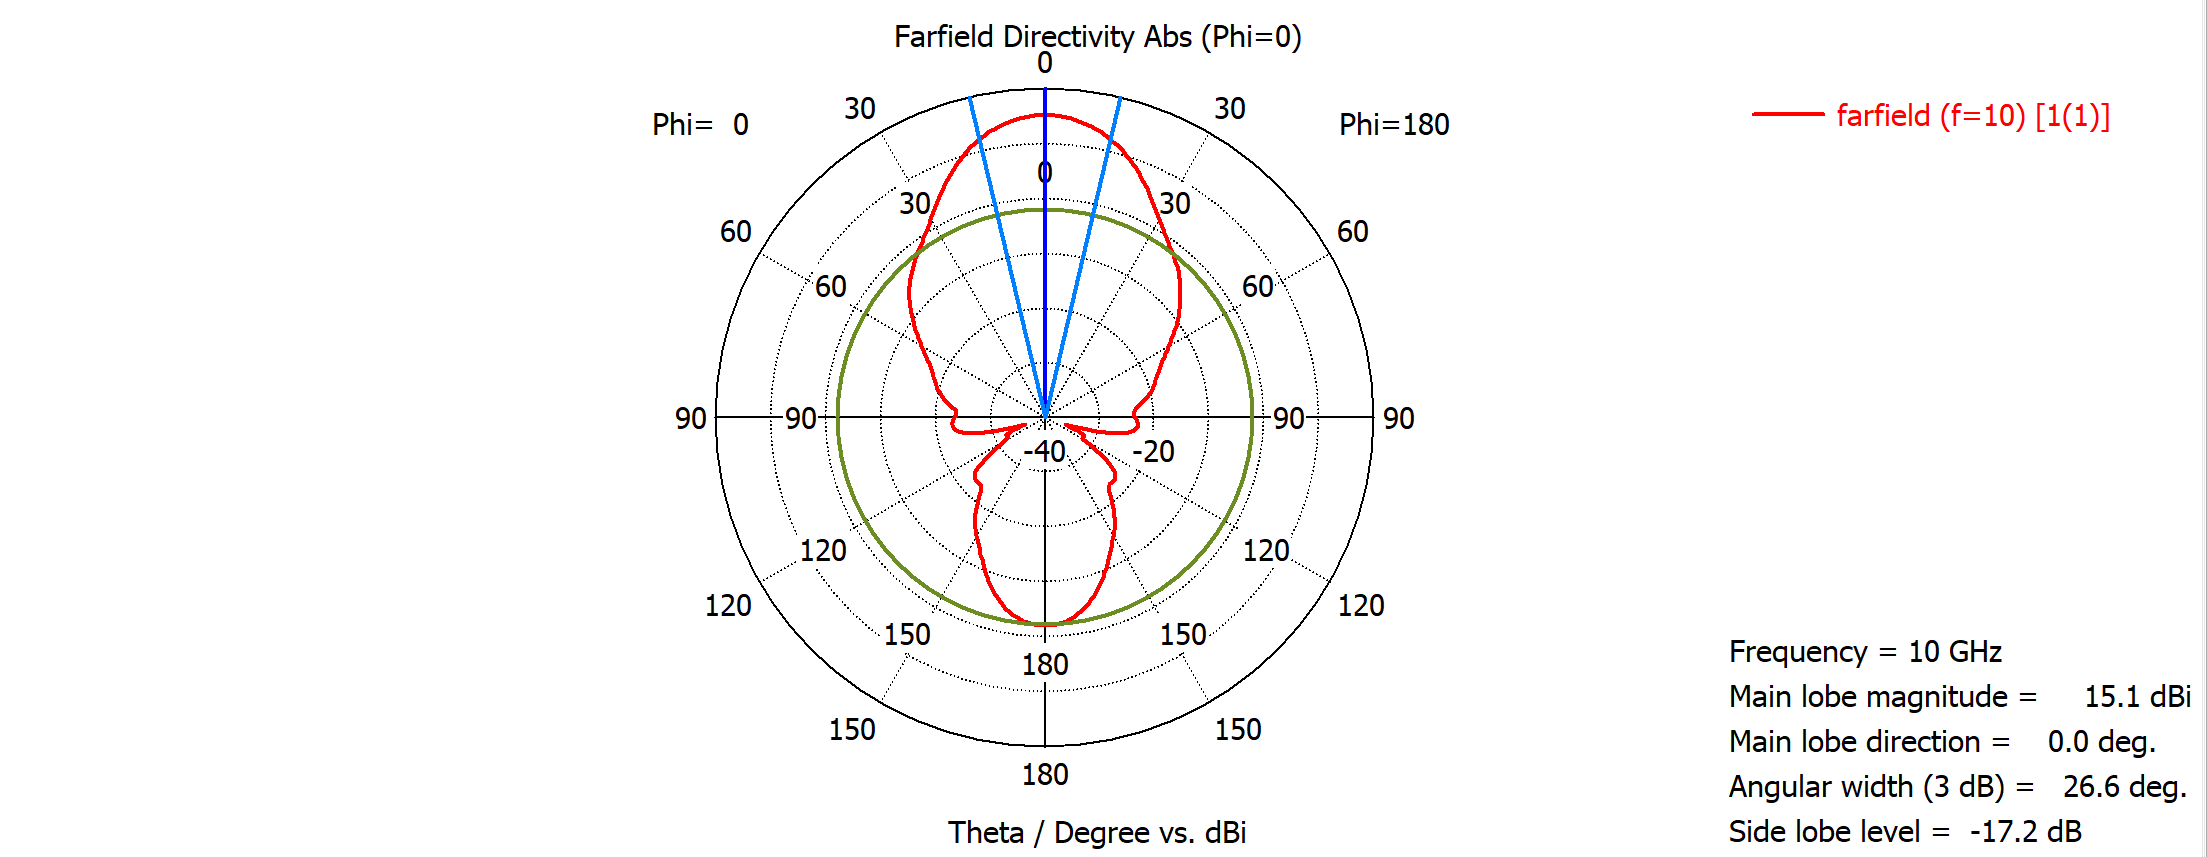
\includegraphics[width=1.0\textwidth]{figures/A23.png}
		\caption{$\phi = 0$方向图}
	\end{minipage}%
	\begin{minipage}[b]{0.5\linewidth}
		\centering
		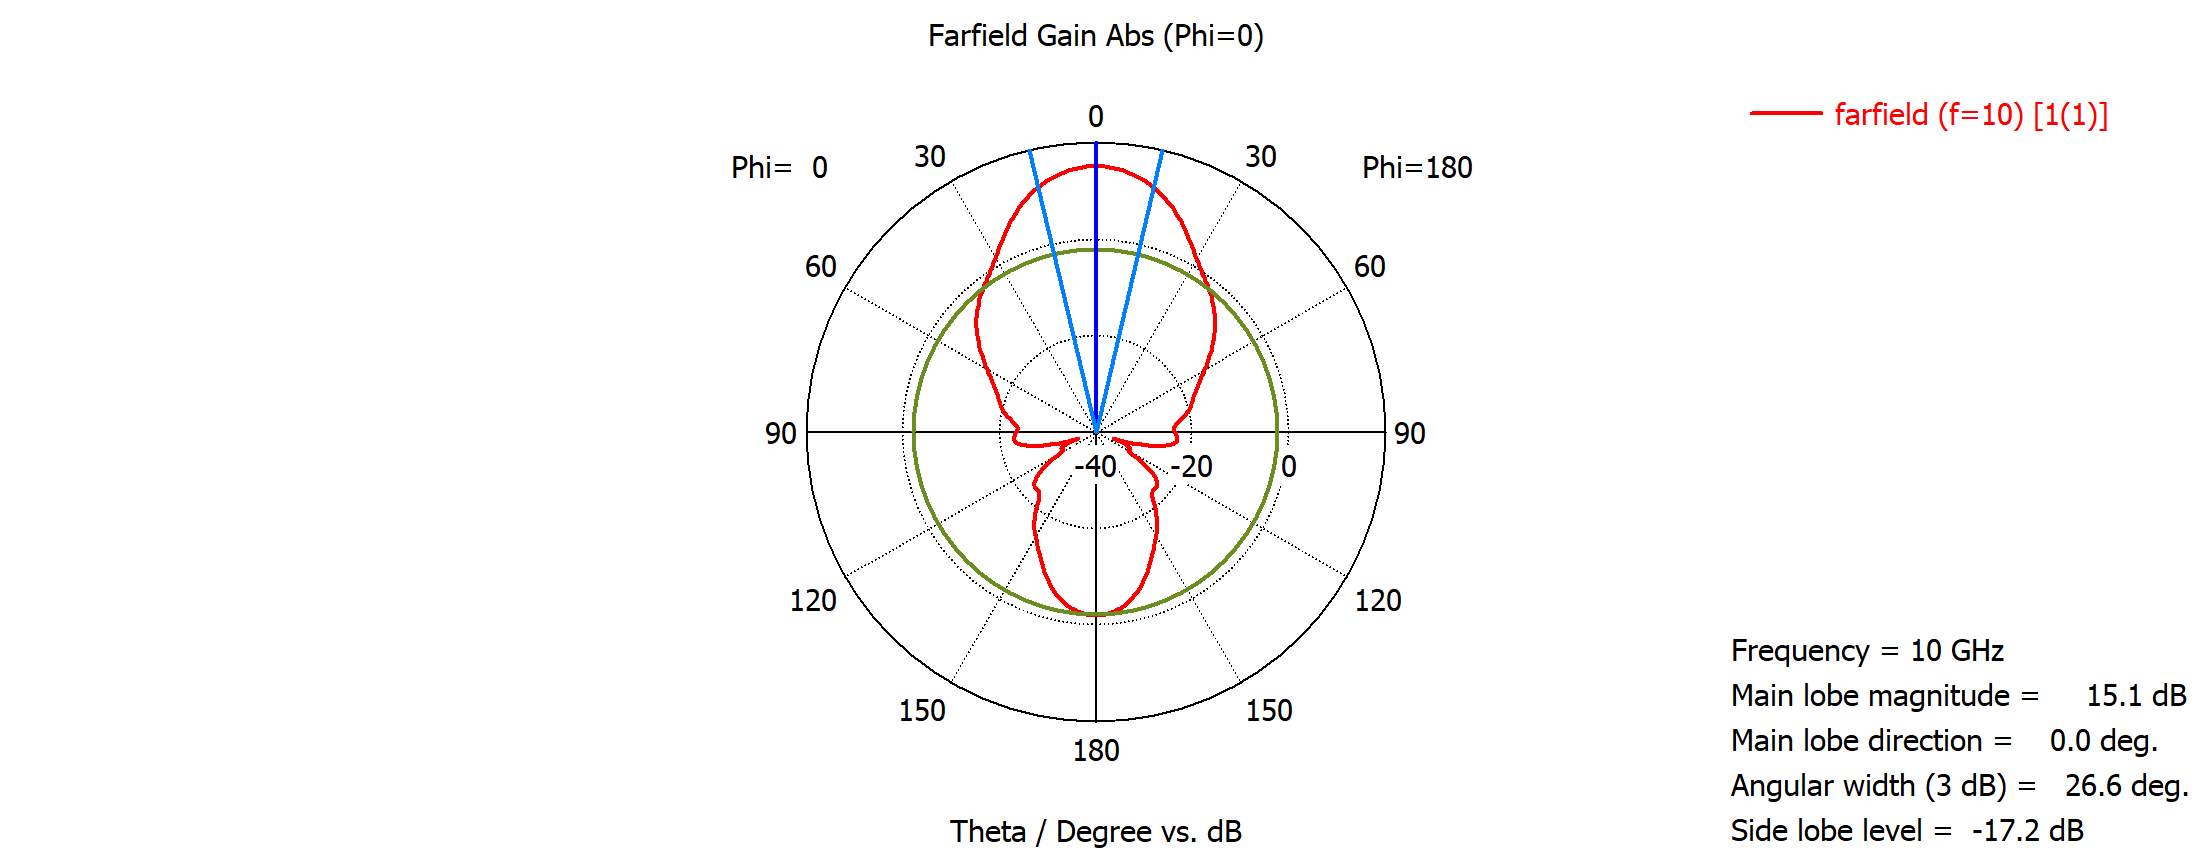
\includegraphics[width=1.0\textwidth]{figures/A23_.png}
		\caption{$\phi = 0$增益图}
	\end{minipage}
\end{figure}
【分析】：$\phi = 0$时，主瓣的方向为0度，最大辐射为15.1 dB。该图的3 dB角宽度为26.6度，副瓣为-17.2 dB，表示主瓣的方向性较强，而副瓣的辐射较小
\begin{figure}[H]
	\centering
	\begin{minipage}[b]{0.5\linewidth}
		\centering
		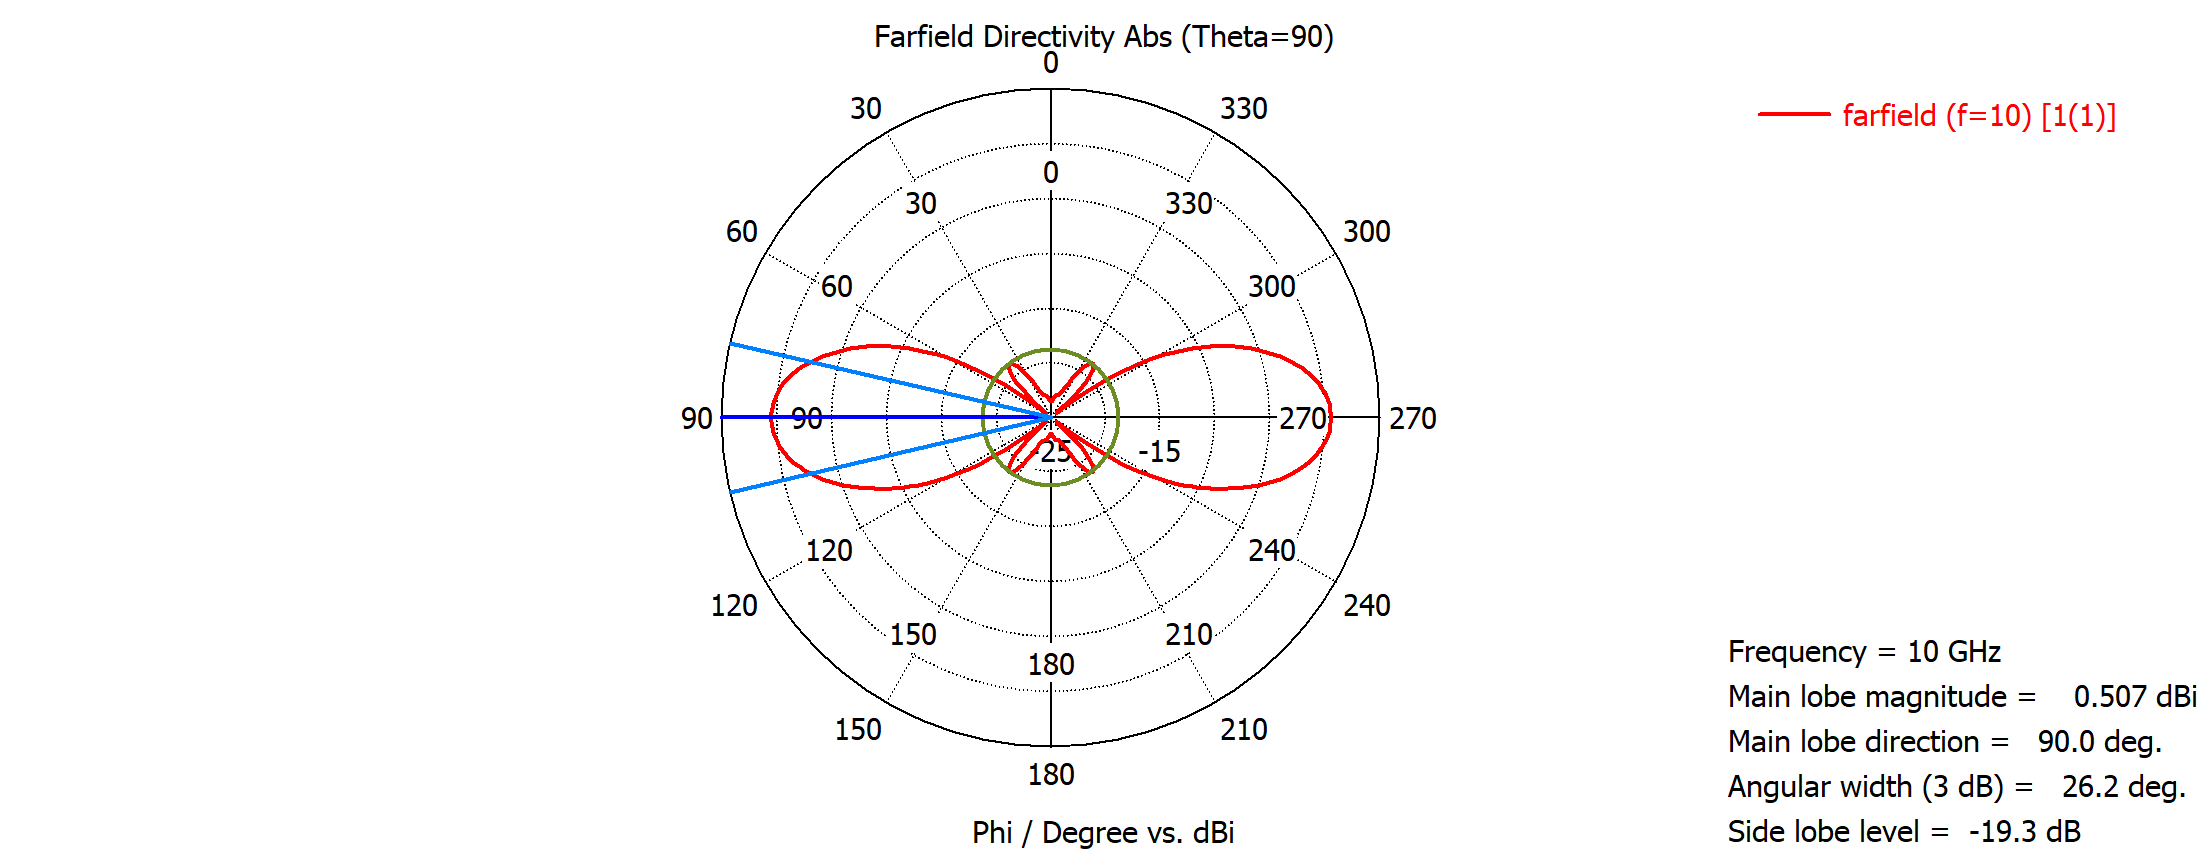
\includegraphics[width=1.0\textwidth]{figures/A24.png}
		\caption{$\theta = 90$方向图}
	\end{minipage}%
	\begin{minipage}[b]{0.5\linewidth}
		\centering
		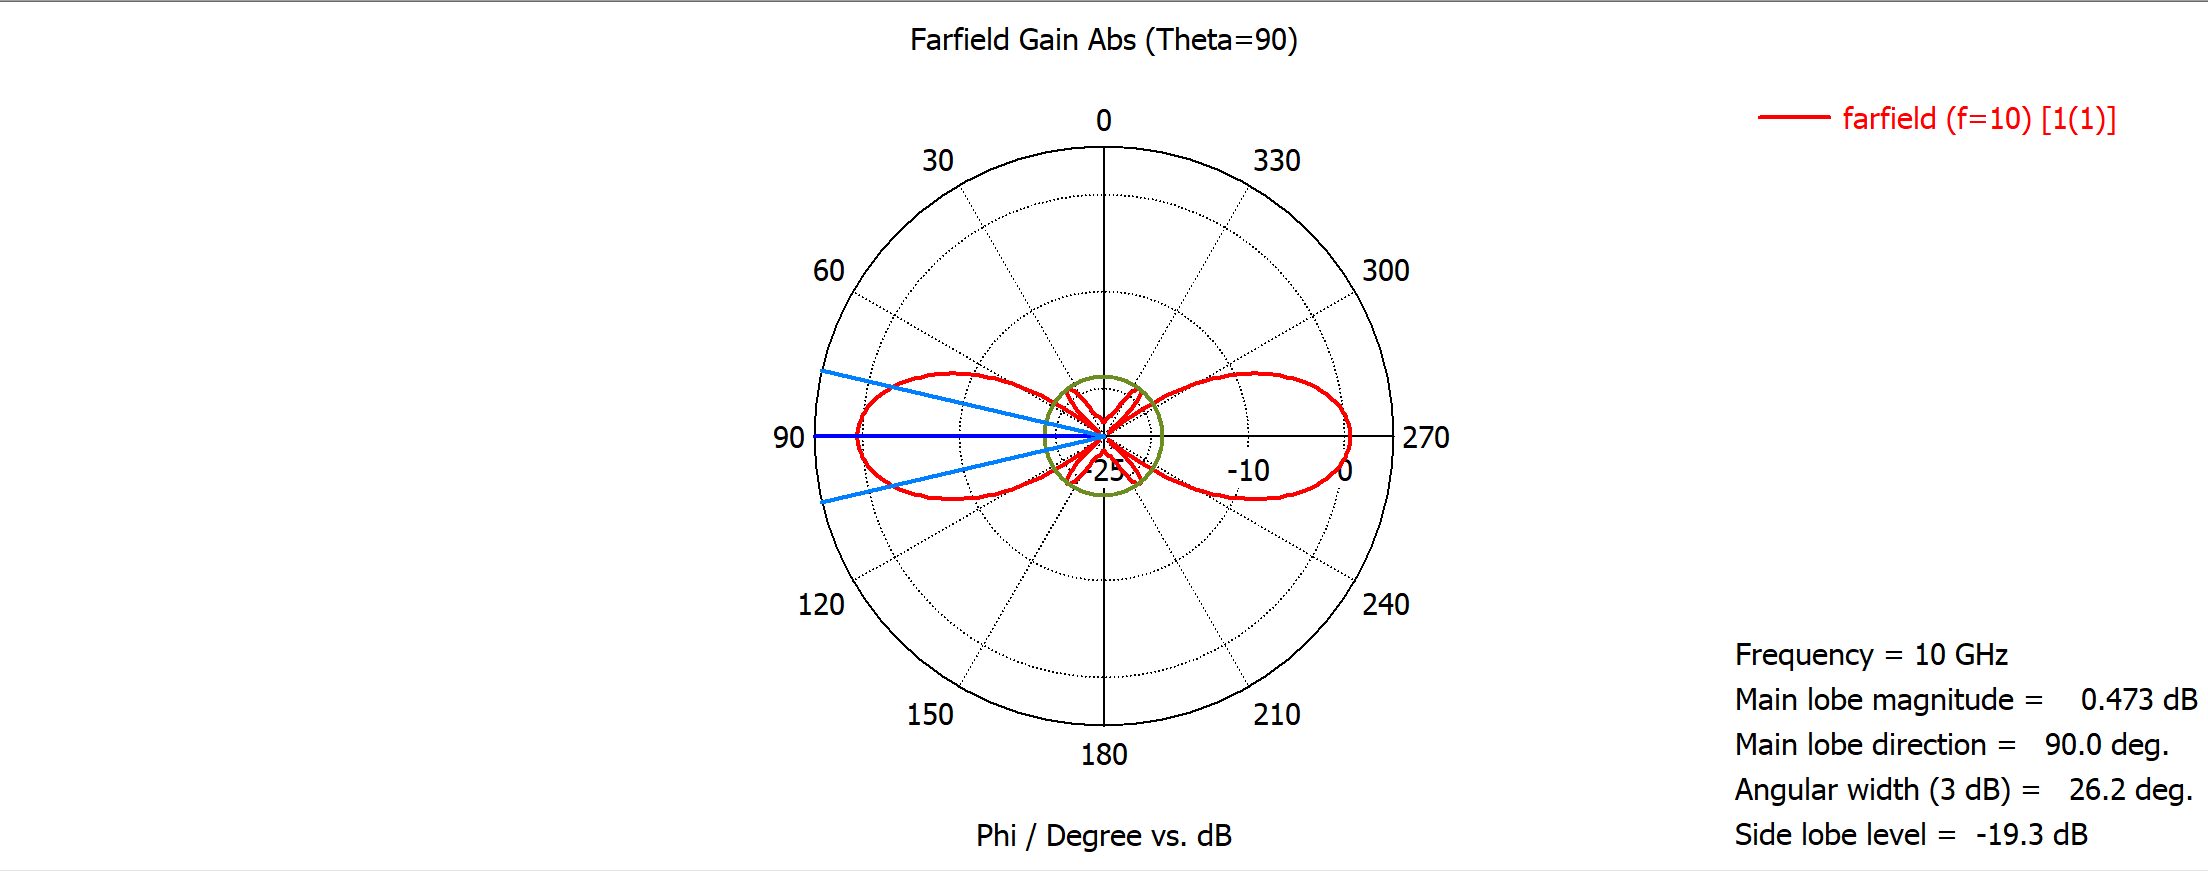
\includegraphics[width=1.0\textwidth]{figures/A24_.png}
		\caption{$\theta = 90$增益图}
	\end{minipage}
\end{figure}
【分析】：$\theta = 90$时，该天线的主瓣方向在90度，最大辐射为0.507 dB,具有一定的3 dB角宽度（26.2度）。侧瓣水平为-19.3 dB，显示了较小的副瓣辐射
\subsection{比较理论增益和仿真结果的异同}

\subsubsection{理论增益计算步骤}

\subsubsection*{参数代入}
\begin{itemize}
    \item \( D_H = 80 \, \text{mm}, \, D_E = 38 \, \text{mm}, \, \lambda = 29.1 \, \text{mm} \)
    \item \( a = 22.86 \, \text{mm}, \, b = 10.16 \, \text{mm}, \, L = 80 \, \text{mm} \)
\end{itemize}

\subsubsection*{计算 \( R_1 \) 和 \( R_2 \)}
\[
R_1 = \frac{L \cdot D_H}{D_H - a} = \frac{80 \times 80}{80 - 22.86} \approx 112.0 \, \text{mm}, \quad
R_2 = \frac{L \cdot D_E}{D_E - b} = \frac{80 \times 38}{38 - 10.16} \approx 109.15 \, \text{mm}.
\]

\subsubsection*{计算 \( L_H \) 和 \( L_E \)}
\[
L_H = \sqrt{R_1^2 + \left(\frac{D_H}{2}\right)^2} = \sqrt{112^2 + 40^2} \approx 119.0 \, \text{mm}, \quad
L_E = \sqrt{R_2^2 + \left(\frac{D_E}{2}\right)^2} = \sqrt{109.15^2 + 19^2} \approx 110.8 \, \text{mm}.
\]

\subsubsection*{计算 \( S_H \) 和 \( S_E \)}
\[
S_H = \frac{a^2}{8 \lambda L_H} = \frac{22.86^2}{8 \times 29.1 \times 119} \approx 0.0189, \quad
S_E = \frac{b^2}{8 \lambda L_E} = \frac{10.16^2}{8 \times 29.1 \times 110.8} \approx 0.0040.
\]

\subsubsection*{计算 \( \alpha \) 和 \( \beta \)}
\[
\alpha = 8S_H \approx 0.1512, \quad \beta = 8S_E \approx 0.032.
\]

\subsubsection*{查表得 \( \Delta G_H \) 和 \( \Delta G_E \)}
    对 \( \alpha = 1.51 \)，查表得：
    \[
    \Delta G_H \approx 0.2603 \, \text{dB}, \quad \Delta G_E = 0.0024 \, \text{dB}.
    \]

	\subsubsection*{计算理论增益}
	\[
	G = 10.8 + 10 \log\left(\frac{D_H \cdot D_E}{\lambda^2}\right) - \Delta G_H - \Delta G_E,
	\]
	其中：
	\[
	\frac{D_H \cdot D_E}{\lambda^2} = \frac{80 \times 38}{29.1^2} \approx 3.59, \quad
	10 \log(3.59) \approx 5.55 \, \text{dB}.
	\]
	最终增益为：
	\[
	G \approx 10.8 + 5.55 - 0.2603 - 0.0024 \approx 16.1 \, \text{dB}.
	\]
\subsubsection{差异分析与原因}
\textbf{增益差异}：理论值（16.1 dB）与仿真值（15.1 dB）总体而言接近，但存在1 dB的差值，猜测主要源于以下因素：
\begin{enumerate}
    \item \textbf{理论模型的简化}：理论公式未考虑天线金属壁损耗、表面粗糙度、端口匹配等实际因素，而仿真模型包含完整的材料属性和边界条件。
    \item \textbf{插值误差}：\(\Delta G_H\) 和 \(\Delta G_E\) 的查表值通过线性插值获得，可能引入精度损失。
\end{enumerate}

\subsection{分析说明喇叭天线和波导口的电场情况}
\begin{enumerate}
	\item 喇叭天线
	\begin{figure}[H]
		\centering
		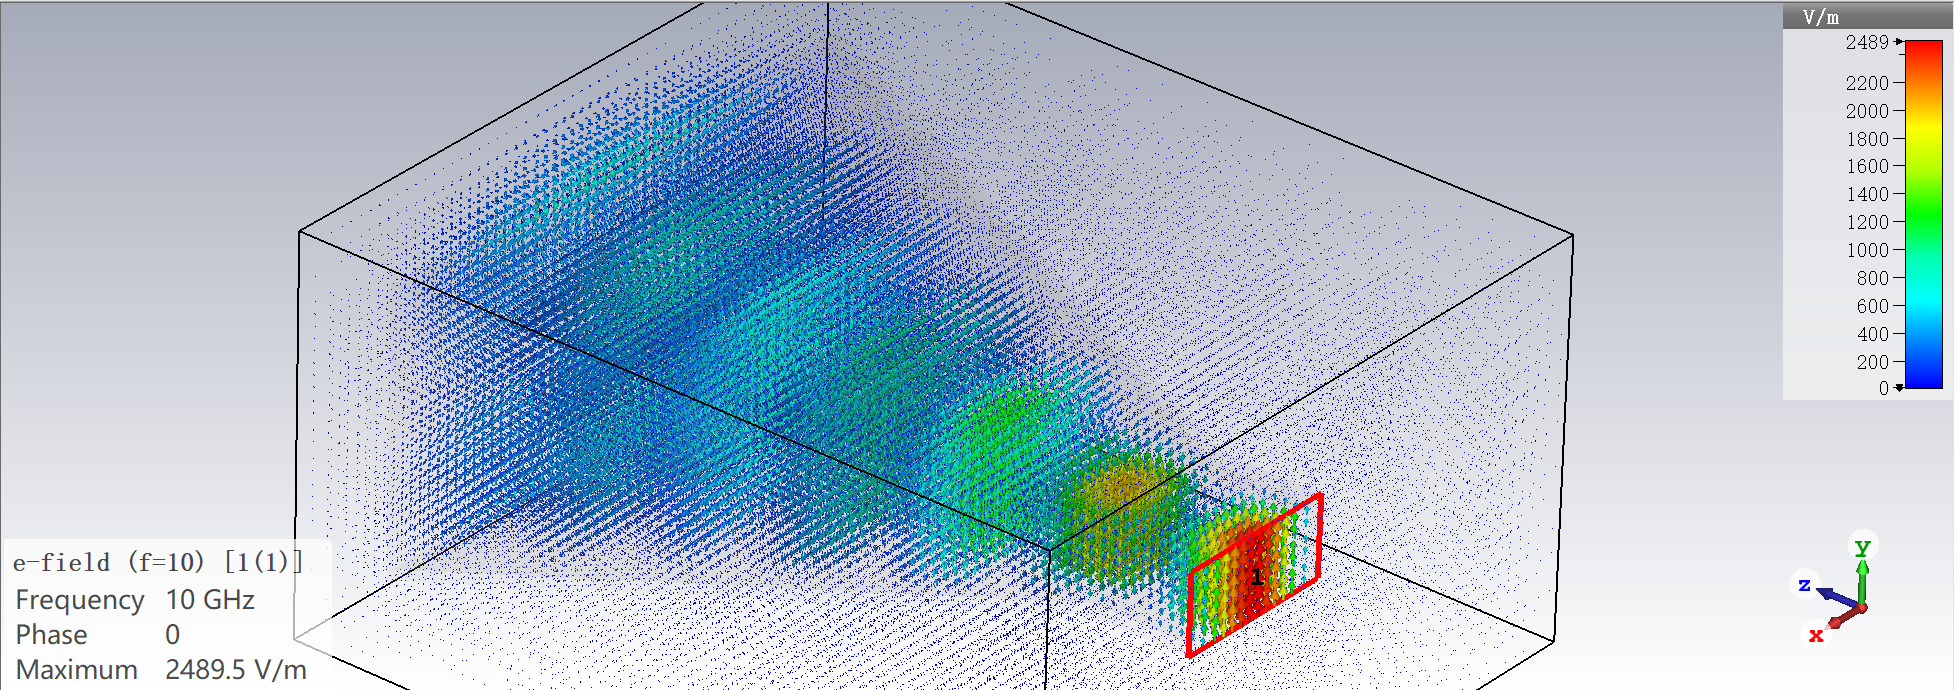
\includegraphics[width=0.65\linewidth]{figures/A41.png} % 数字表示放缩比例
		\caption{喇叭天线电场情况} % 图片标题
	\end{figure}
【分析】：图中小箭头表示电场的方向，颜色深度代表电场强度。从图中可见，电场强度以Y轴对称，在天线端口中心位置最强，最大值约为2489.5 V/m，表明能量集中在该区域。随着距离天线端口的增大，电场强度逐渐减小，边缘位置电场强度较低。
	\item 波导口
	\begin{figure}[H]
		\centering
		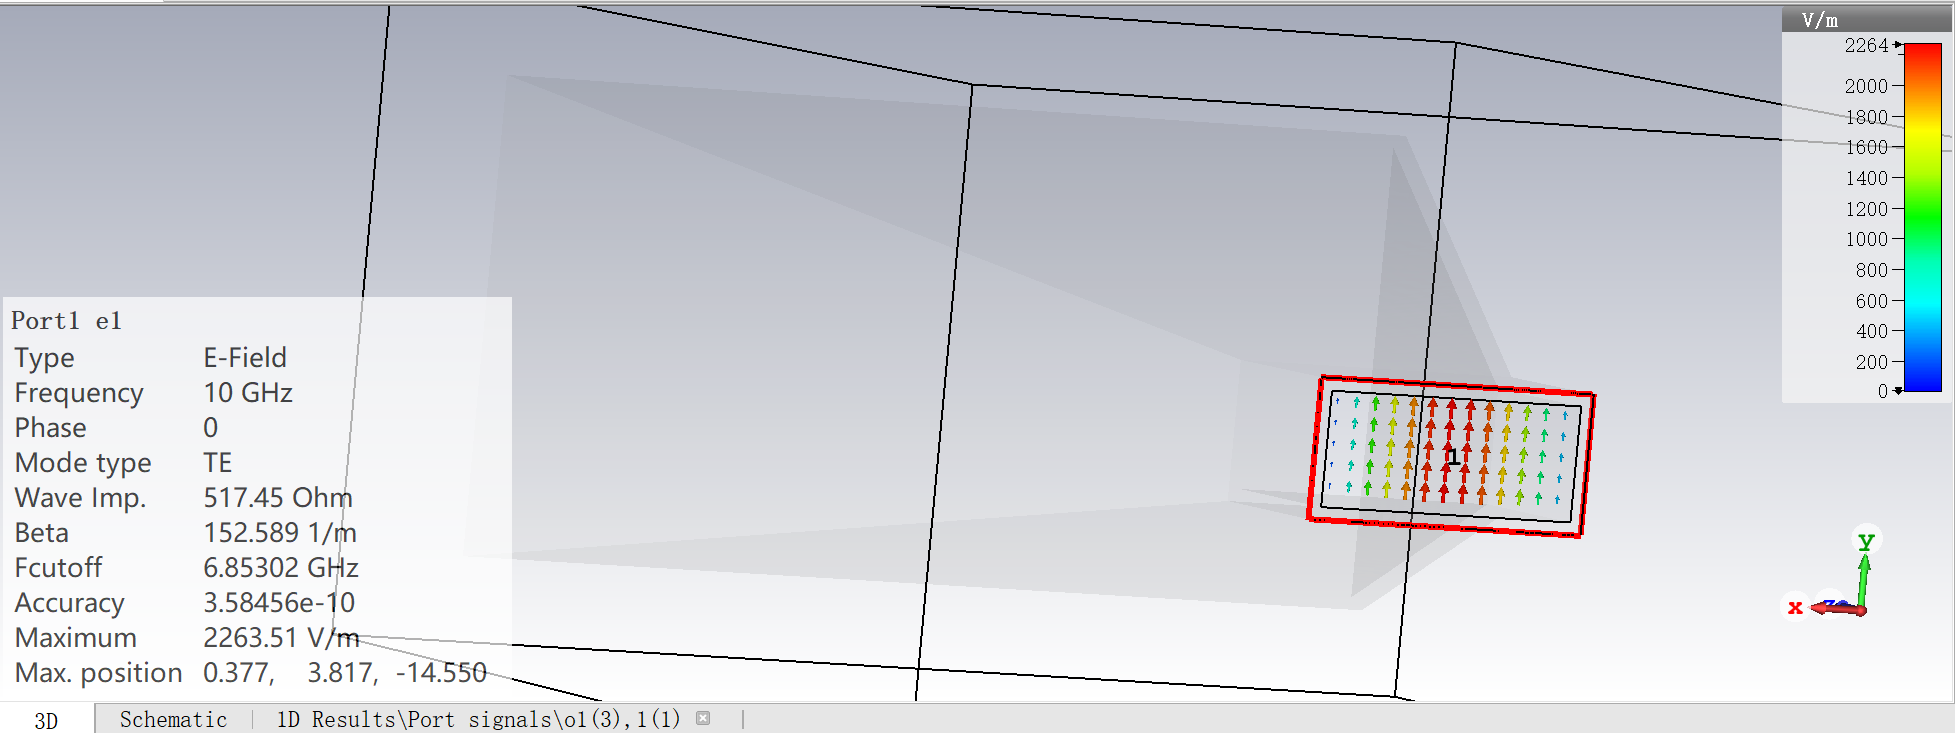
\includegraphics[width=0.65\linewidth]{figures/A44.png} % 数字表示放缩比例
		\caption{波导口电场情况} % 图片标题
	\end{figure}
【分析】：端面电场指向Y方向并以Y轴对称，最大电场强度为2263.51 V/m，电场强度在端面中心最强，向两侧扩展时电场强度逐渐减小。
	\end{enumerate}
\subsection{分析说明喇叭天线和波导口的磁场情况}
\begin{enumerate}	
	\item 喇叭天线
	\begin{figure}[H]
		\centering
		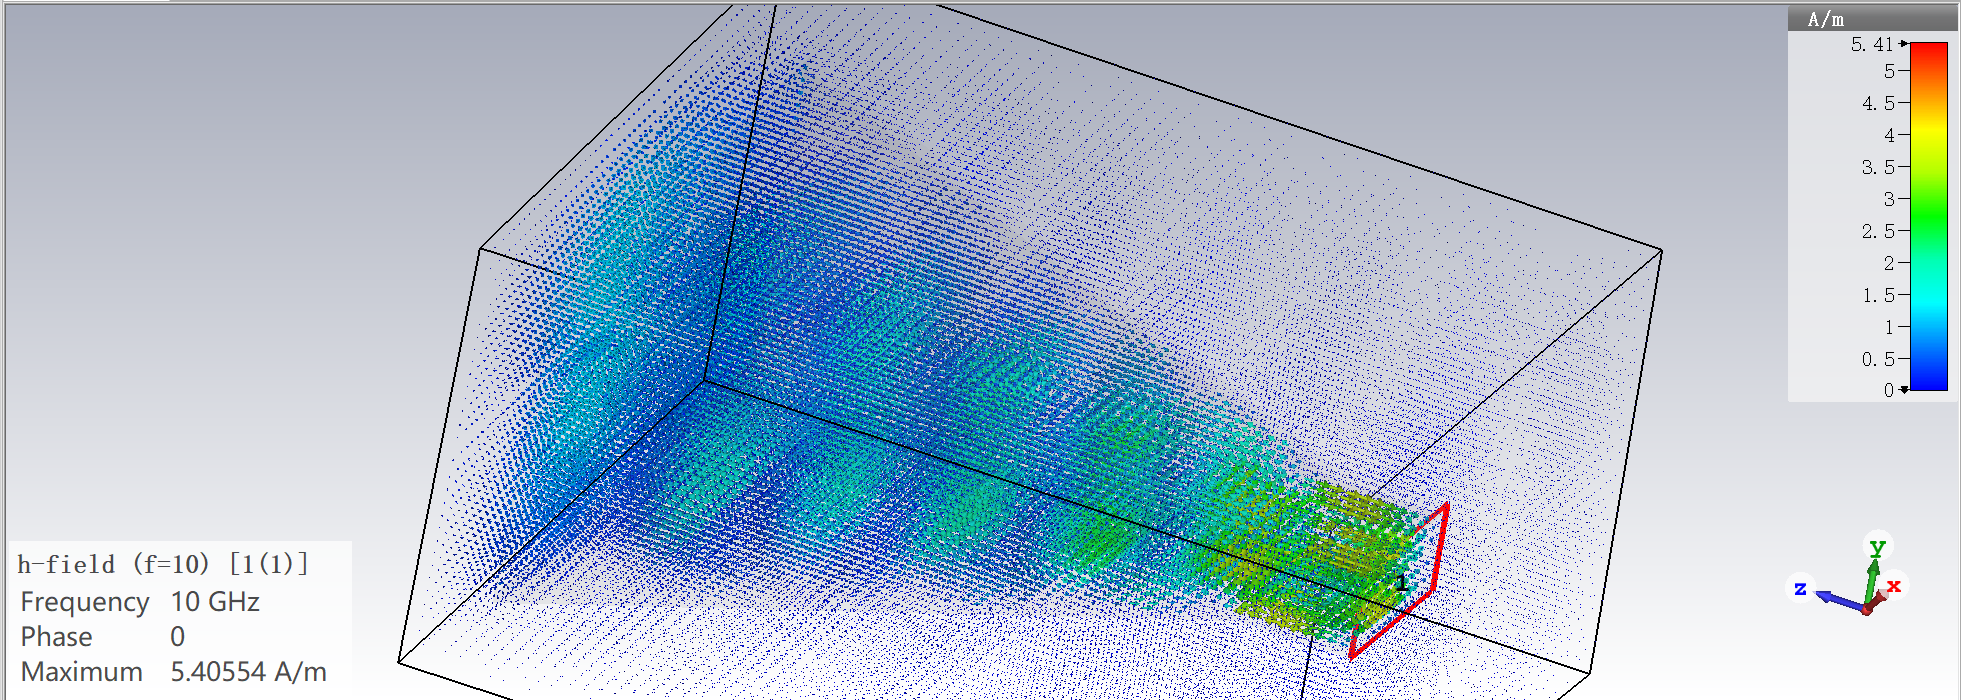
\includegraphics[width=0.65\linewidth]{figures/A42.png} % 数字表示放缩比例
		\caption{喇叭天线磁场情况} % 图片标题
	\end{figure}
【分析】：小箭头显示了磁场方向，颜色深度表示磁场强度。最大值为5.41 A/m，磁场在天线端口处最强，随着距离增大逐渐减弱，显示出磁场的辐射特性。
	\begin{figure}[H]
		\centering
		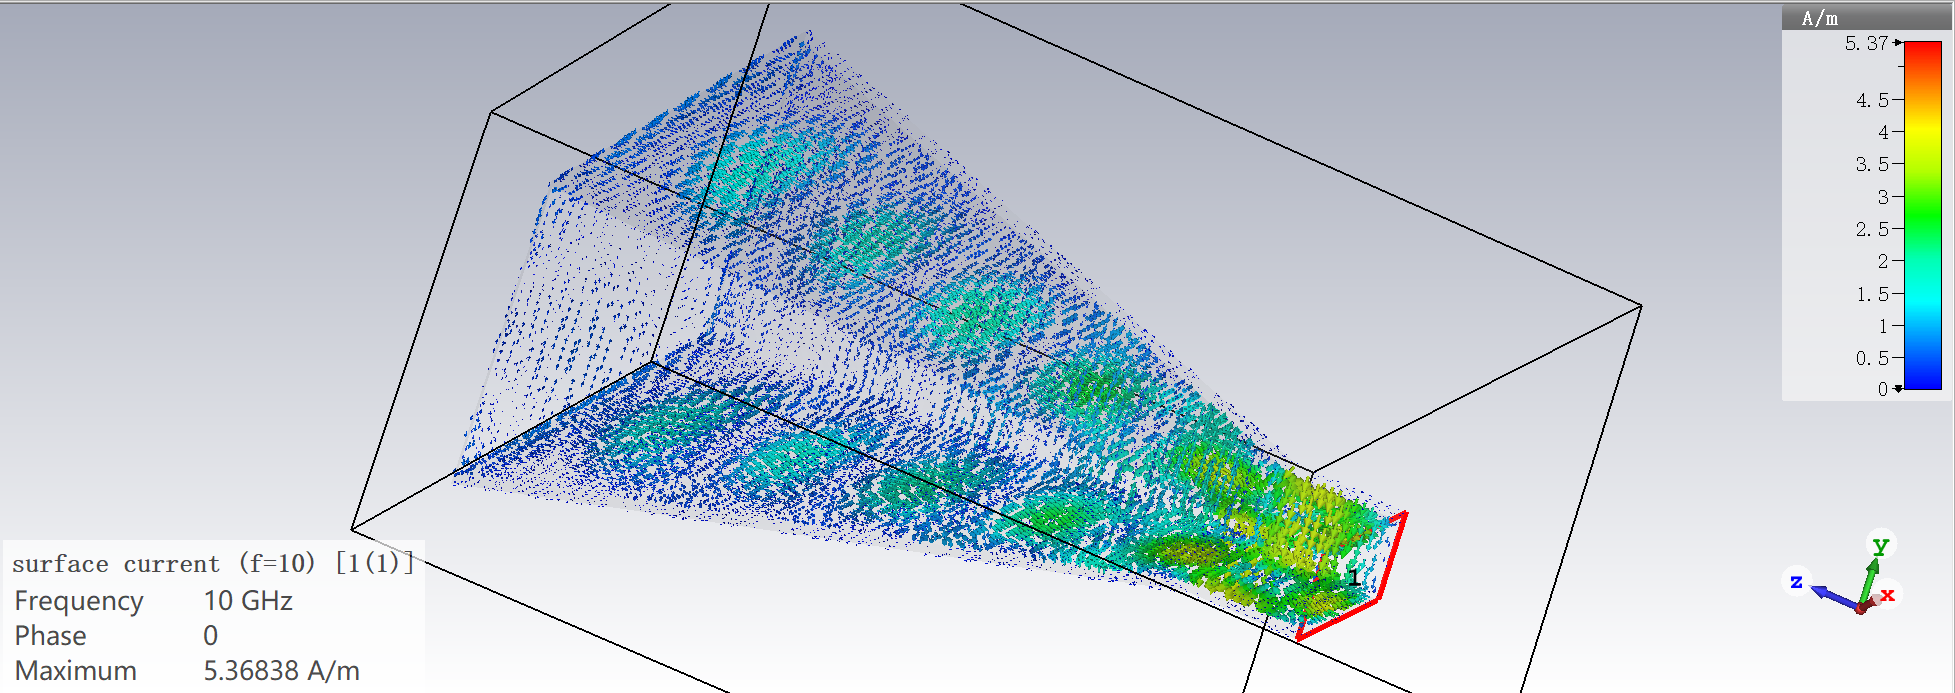
\includegraphics[width=0.65\linewidth]{figures/A43.png} % 数字表示放缩比例
		\caption{喇叭天线表面电流情况} % 图片标题
	\end{figure}
【分析】：最大电流为5.37 A/m，电流在天线表面集中的区域较强，随着距离增大，电流逐渐衰减，表明电流的传播方向性。
	\item 波导口
	\begin{figure}[H]
		\centering
		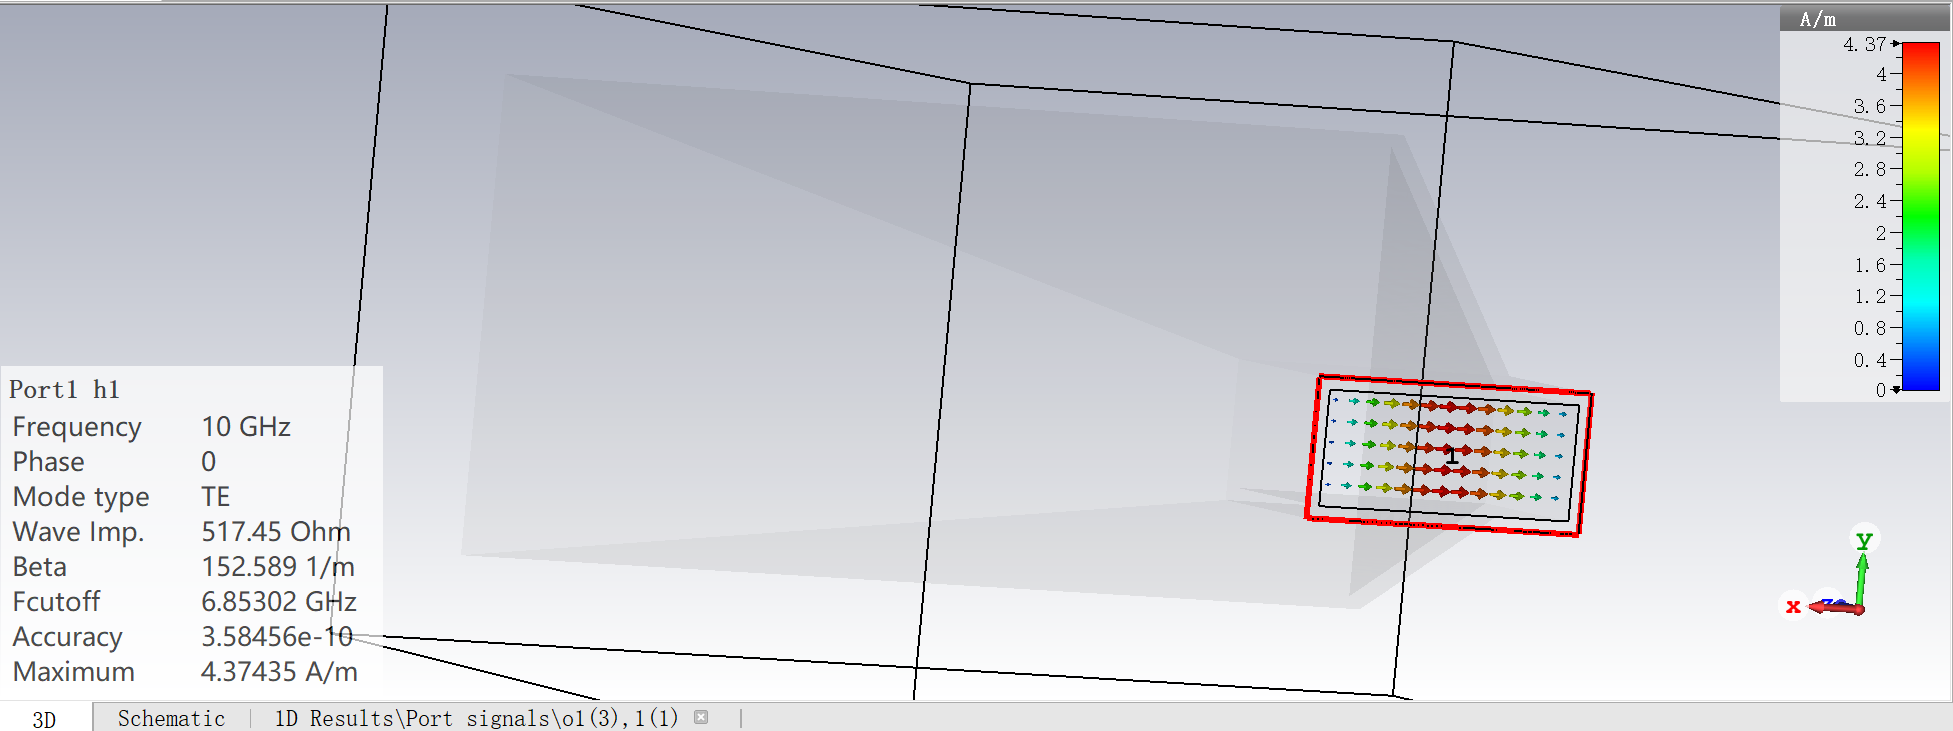
\includegraphics[width=0.65\linewidth]{figures/A45.png} % 数字表示放缩比例
		\caption{波导口磁场情况} % 图片标题
	\end{figure}
【分析】：波导口磁场指向-X方向，磁场大小以Y轴对称，最大值为4.37 A/m，磁场在端面中心密集，向两侧逐渐减弱。
\end{enumerate}
\section{实验的收获与体会}
\subsection{实验收获}  
\begin{enumerate}
    \item \textbf{加深了对喇叭天线工作原理的理解}  
    \begin{itemize}
        \item 通过本次实验，深入了解了矩形波导、角锥喇叭天线的结构特点和工作原理。喇叭天线通过逐渐扩展波导口径实现阻抗匹配，减少了反射，提高了辐射效率。实验过程中，通过理论分析和仿真验证，进一步掌握了喇叭天线的增益计算方法和方向图特性。
    \end{itemize}

    \item \textbf{熟悉了CST仿真软件的操作流程}  
    \begin{itemize}
        \item 从建模到仿真，学习了CST软件的基本操作，包括参数设置、几何建模、边界条件配置、端口设置以及结果分析。尤其是通过实际动手操作，掌握了如何创建复杂的喇叭天线模型，并对其性能进行仿真分析。
    \end{itemize}

    \item \textbf{理论与实践的结合}  
    \begin{itemize}
        \item 通过对比理论增益公式（$G = 10.8 + 10\lg(D_H \times D_E / \lambda^2) - \Delta G_H - \Delta G_E$）与仿真结果，发现两者较为接近，验证了理论分析的正确性。同时，也认识到仿真中可能存在的误差来源，如边界条件设置、网格划分精度等。
    \end{itemize}

    \item \textbf{掌握了天线性能的分析方法}  
    \begin{itemize}
        \item 学会了如何通过仿真结果分析天线的关键性能指标，如：
        \begin{itemize}
            \item \textbf{S11参数和驻波比}：判断天线的阻抗匹配情况。
            \item \textbf{方向图}：分析天线的辐射特性，包括主瓣宽度、副瓣电平、方向性等。
            \item \textbf{增益和效率}：评估天线的辐射性能。
            \item \textbf{电场和表面电流分布}：了解天线的工作状态和能量分布。
        \end{itemize}
    \end{itemize}

    \item \textbf{提升了问题解决能力}  
    \begin{itemize}
        \item 在建模和仿真过程中，遇到了一些问题（如端口设置错误、边界条件不合理等），通过查阅资料和反复调试，最终解决了这些问题。这一过程增强了独立分析和解决问题的能力。
    \end{itemize}

\end{enumerate}

\subsection{实验体会}  
本次实验不仅巩固了理论知识，还提升了实践能力和软件操作技能，促使我更努力的去学习《电磁场与电磁波》课程。同时，也让我认识到仿真工具在工程实践中的重要性，以及理论与实际结合的必要性。
\end{document}
